\documentclass{article}

% if you need to pass options to natbib, use, e.g.:
% \PassOptionsToPackage{numbers, compress}{natbib}
% before loading nips_2017
%
% to avoid loading the natbib package, add option nonatbib:
% \usepackage[nonatbib]{nips_2017}

%\usepackage{icml2019}
\usepackage[accepted]{icml2019}

% to compile a camera-ready version, add the [final] option, e.g.:
% \usepackage[final]{nips_2017}

\usepackage[utf8]{inputenc} % allow utf-8 input
\usepackage[T1]{fontenc}    % use 8-bit T1 fonts
%\usepackage{hyperref}       % hyperlinks
\usepackage{url}            % simple URL typesetting
\usepackage{booktabs}       % professional-quality tables
\usepackage{amsfonts}       % blackboard math symbols
\usepackage{nicefrac}       % compact symbols for 1/2, etc.
\usepackage{microtype}      % microtypography
\usepackage{amssymb}
\usepackage{amsmath}
\usepackage{mathabx}
\usepackage{optidef}
\usepackage{xcolor}
\usepackage{multirow}
\usepackage{bbm}
\usepackage{caption}
\usepackage{subcaption}
\usepackage{enumitem}

\usepackage{appendix}
%\usepackage{etoolbox}
% Inserts \clearpage before every \section within appendices environment
%\AtBeginEnvironment{appendices}{\pretocmd{\section}{\clearpage}{}{}}{}

% Attempt to make hyperref and algorithmic work together better:
\newcommand{\theHalgorithm}{\arabic{algorithm}}

\usepackage{array,tabularx}
\newenvironment{vardefs*}{\par\vspace{\abovedisplayskip}\noindent
	\tabularx{\columnwidth}{>{$}l<{$} @{${}:{}$} >{\raggedright\arraybackslash}X}}
{\endtabularx\par\vspace{\belowdisplayskip}}

\everymath{\displaystyle} 

\icmltitlerunning{ORL: Reinforcement Learning Benchmarks for Online Stochastic Optimization Problems}
%s\title{Benchmarks for Online Stochastic Operations Research Problems}

\begin{document}

\twocolumn[
\icmltitle{ORL: Reinforcement Learning Benchmarks for Online Stochastic Optimization Problems}

% It is OKAY to include author information, even for blind
% submissions: the style file will automatically remove it for you
% unless you've provided the [accepted] option to the icml2019
% package.

% List of affiliations: The first argument should be a (short)
% identifier you will use later to specify author affiliations
% Academic affiliations should list Department, University, City, Region, Country
% Industry affiliations should list Company, City, Region, Country

% You can specify symbols, otherwise they are numbered in order.
% Ideally, you should not use this facility. Affiliations will be numbered
% in order of appearance and this is the preferred way.
\icmlsetsymbol{equal}{}

\begin{icmlauthorlist}
	\icmlauthor{Bharathan Balaji}{equal,to}
	\icmlauthor{Jordan Bell-Masterson}{equal,to}
	\icmlauthor{Enes Bilgin}{equal,to}
	\icmlauthor{Andreas Damianou}{equal,to}
	\icmlauthor{Pablo Moreno Garcia}{equal,to}
	\icmlauthor{Arpit Jain}{equal,to}
	\icmlauthor{Runfei Luo}{equal,to}
	\icmlauthor{Alvaro Maggiar}{equal,to}
	\icmlauthor{Balakrishnan Narayanaswamy}{equal,to}
	\icmlauthor{Chun Ye}{equal,to}
	%Others please add your names
\end{icmlauthorlist}

\icmlaffiliation{to}{Amazon.com, Inc.}
%\icmlaffiliation{goo}{SCOT SimEx}
%\icmlaffiliation{ed}{GDS MOP}

\icmlcorrespondingauthor{Bharathan Balaji}{bhabalaj@amazon.com}

% You may provide any keywords that you
% find helpful for describing your paper; these are used to populate
% the "keywords" metadata in the PDF but will not be shown in the document
\icmlkeywords{reinforcement learning, benchmarks, operations research, online stochastic optimization, bin packing, vehicle routing, newsvendor}

\vskip 0.3in
]

\setlength{\abovedisplayskip}{3pt}
\setlength{\belowdisplayskip}{3pt}

\printAffiliationsAndNotice{}  % leave blank if no need to mention equal contribution
%\printAffiliationsAndNotice{\icmlEqualContribution} % otherwise use the standard text.


%\maketitles
	
\begin{abstract}
 Reinforcement Learning (RL) has achieved state-of-the-art performance in domains such as robotics and games.  We build on this previous work by applying RL algorithms to a selection of canonical online stochastic optimization problems with a range of practical applications: Bin Packing, Newsvendor, and Vehicle Routing.  While there is a nascent literature that applies RL to these problems, there are no commonly accepted benchmarks which can be used to compare proposed approaches rigorously in terms of performance, scale, or generalizability. This paper aims to fill that gap.  For each problem, we apply both well-known approaches and newer RL algorithms and analyze results.  In each case, the performance of the trained RL policy is competitive with or superior to the corresponding baselines, pointing the way for future research on applying RL to real-world online stochastic optimization problems and algorithmic improvements. 
% The domain of Operations Research (OR) is particularly amenable to RL approaches since many of the canonical problems can be characterized as online stochastic optimization problems where the distribution of data is unknown.  
% Canonical online stochastic optimization (OSO) problems in Operations Research (OR) are particularly amenable to RL approaches, especially where the distribution of data is unknown. 
%While there is a nascent literature that applies RL to these problems, there are no commonly accepted benchmarks which can be used to compare proposed approaches rigorously in terms of performance, scale, or generalizability. This paper aims to fill that gap by introducing open source %OR+RL  benchmarks for three canonical OSO problems with a wide range of practical applications: Bin Packing, Newsvendor, and Vehicle Routing. We apply both well-known approaches and newer RL algorithms to these problems and analyze results.  For each problem, the performance of trained RL policy is competitive with or superior to the corresponding baselines, pointing the way for future research on applying RL to real world OSO problems and algorithmic improvements.
\end{abstract}

\section{Introduction}

Reinforcement learning (RL) has gained steam in recent years with state of the art results in gaming~\cite{mnih2013playing,silver2017mastering}, robotics~\cite{hwangbo2019learning,andrychowicz2018learning}, computing~\cite{mao2017neural, marcus2018towards,mirhoseini2017device}, recommendation systems~\cite{chen2019top,zhao2018deep}, and many others. In RL, an agent interacts with an environment in a Markov Decision Process (MDP). The agent takes actions with the environment state as input and receives a scalar reward and the next state. RL algorithms learn a policy that maximizes the cumulative discounted reward from repeated interactions with the environment. Classic RL algorithms, such as Q-learning~\cite{watkins1992q}, require visitation to every discrete state, action pair for convergence. However, with the use of neural networks, RL can learn compact state representations and successful policies for high-dimensional state spaces~\cite{riedmiller2005neural,mnih2013playing}. With enough interactions, state-of-the-art RL algorithms can learn to make intelligent decisions that even beat human strategies~\cite{silver2017mastering}.

%Challenging problems in operations research fall into one of two categories: 1) large scale combinatorial optimization problems, where computing an optimal solution requires clever enumeration through a large discrete set. 2) multi-period stochastic optimization problems, where the problem state space increases exponentially with the length of the time horizon. 
%Many recent works have shown promising results applying RL to optimization problems. 
Our work relates to the growing literature of applying RL to optimization problems. \citet{bello2016neural} show RL techniques produce near optimal solutions for the traveling salesman (TSP) and knapsack problems. \citet{kool2018attention} use RL to solve TSP and its variants: vehicle routing, orienteering, and a stochastic variant of prize-collecting TSP. \citet{nazari2018reinforcement} solve both static and online versions of the vehicle routing problem. \citet{gijsbrechts2018can} apply RL to the dual sourcing inventory replenishment problem, and further demonstrate results on a real dataset. \citet{kong2018new} apply RL to online versions of the knapsack, secretary and adwords problems. \citet{oroojlooyjadid2017deep} apply RL to the beer game problem. \citet{lin2018efficient} use RL for fleet management of taxis on a real life dataset. 
%These works show that RL can get close to known optimal solutions for static versions of the problems. 

%State-of-the-art OR solutions are often near optimal for static versions of these problems. For online stochastic versions of these problems, however, OR approaches often make assumptions on input distributions or convexity of the problem in their formulation. The RL approach can learn the distribution based on data and make end-to-end optimization decisions that maximize the long term objective. Early results in literature are promising, but there exist no benchmarks for the online stochastic optimization problems to rigorously compare algorithms in terms of performance, scale, generalizability and, in case of RL, training time. 

Our contribution is to extend the existing RL literature to a set of online stochastic optimization problems with parallels to real-world problems. In particular, we present benchmarks for three classic problems: Bin Packing, Newsvendor and Vehicle Routing.  In each case, we show that trained policies from out-of-the-box RL algorithms with simple 2 layer neural networks and default hyper-parameters are competitive with or superior to established approaches to these problems. 
We aim to spur further work in two directions.  First, we open source our code and parameterize the complexity of the problems in order to encourage fair comparisons of algorithmic contributions.  Each environment is implemented with OpenAI Gym interface~\cite{brockman2016openai} and integrated with RLlib~\cite{liang2017rllib} library so researchers can easily test multiple algorithms and tune hyper-parameters. %Second, we highlight the close parallels between these problem formulations and a host of practical problems, showing how further research can directly impact production scenarios.
Second, since RL learns from exploratory actions, future work can focus on building effective simulators and learning from historical data to apply RL in real world scenarios.
%Each problem has been implemented with a standard OpenAI Gym interface and parameterized so we can change the complexity of the problem. We have implemented well known baselines solutions and compare them with the performance of RL algorithms. We will open source our code for reproducibility and development of better algorithms by the community.

% RL is a good fit
%% learns the distribution
%% end to end approach
% OR papers with RL
% online stochastic problems are harder than NP hard
% No benchmarks

%Operations Research is an awesome field. Many online stochastic problems exist in practice but solutions make simplistic assumption. Reinforcement learning is a good fit to these problems and there have been some initial results. However, no standard set of problems or algorithms to compare against exist. We prepare these benchmarks to compare different algorithms and push the community towards developing better ones. 

%\section{Related Work}

\section{Bin Packing}
\label{binpacking}

In the classic version of the problem, we are given items of different sizes and need to pack them into as few bins as possible. In the online stochastic version, items arrive one at a time and item sizes are drawn from an unknown distribution. 
Many resource allocation problems in Operations Research and Computer Science face uncertain future demand, and can be cast as variants of the online bin packing problem. In warehouse and transportation operations, variants of bin packing can be seen in: the order assignment problem (where we assign orders to fulfillment resources), the tote packing problem (where we fill items as they arrive into totes for shipment), and the trailer truck packing problem. In computing, bin packing problems arise in datacenters where virtual machines must be placed on servers, thus allocating memory and computing to processes within a machine.


%For instance, in the cutting stock problem, a manufacturer produces cables of fixed lengths, customer orders that with specific cable lengths arrive and must be served online from the available inventory.  The goal is to serve the demand while minimizing the rate of production of cables. In appointment scheduling, requests for appointments arrive online and must be scheduled in a future day with available slots. Here appointments correspond to items, and the office hours during a working day correspond to bins. 

%In this problem, customers orders arrive online and must be assigned to a ship method that connects an Amazon FC to the customer's location. For candidate each assignment, the order items would utilize our transportation resources (truck/plane space, labor). The task is to fulfill all orders while utilizing the least number of transportation resources.
 
\ifx 3d bin packing has many applications within Amazon operations from packing of picked items into totes to the packing of packages onto trailers. The need to use as few bins as possible directly translates into cost savings. \emph{Bharath} can you write about the VM
\fi

\subsection{Problem Formulation} \label{sec: bin_packing_prob_form}
In the stochastic bin packing problem, items arrive online, one in each time period $t$, with $t \in \{1, \ldots, T\}$. Items can be of different types $j \in \{1,...,J\}$. The size of type $j$ is $s_j$ and the probability that an item is of type $j$ is $p_j$. Without loss of generality, we assume item types are indexed in the increasing order of their size: $s_1 < s_2 < ... < s_J$. Upon arrival, the item needs to be packed into one of the bins, each with size $B$ (we assume that $s_J < B < \infty$). A packing is considered feasible if the total size of the items packed in each bin does not exceed the bin size. The task is to find a feasible packing that minimizes the number of bins used to pack all of the items that arrive within the time horizon. We assume the item sizes $s_j$ and bin size $B$ are integers. We assume the number of bins one can open is unlimited and denote the sum of item sizes in a bin $k$ as \emph{level} $h_{k}$. After $t$ items have been packed, we denote the number of bins at some level $h$ as $N_h(t)$, where $h \in \{1,...,B\}$. The formulation of online bin packing is from \cite{gupta2012online}. 

It can be shown that minimizing the number of non-empty bins is equivalent to minimizing the total waste (i.e. empty space) in the partially filled bins.  In real applications (e.g. packing trucks, or virtual machines), there is a dollar-value cost associated with the consumption of these resources, so at any time horizon our objective is to minimize total waste $\sum_{t=0}^{T} W(t)$, where

\begin{equation}
\label{waste}
W(t) \triangleq \sum_{h=1}^{B-1} N_h(t)(B-h) 
\end{equation}

\noindent We use $W^{A}_{F}(t)$ to denote the total waste after step $t$ of algorithm $A$ when the input samples come from distribution $F$. For RL, we define the cumulative reward up to time step $t$ to be $W^{RL}_{F}(t)$. \cite{courcobetis1990stability} showed that any discrete distribution falls into one of three categories based on expected distribution $E[W^{OPT}_{F}(t)]$.
\begin{enumerate}[topsep=0pt,itemsep=-1ex,partopsep=1ex,parsep=1ex]
	\item Linear waste (LW): $E[W^{OPT}_{F}(t)] = \Theta(t)$, e.g. $B = 9$, two item types of size $\{2,3\}$ with probability $\{0.8, 0.2\}$ respectively.
	\item Perfectly Packable (PP):  $E[W^{OPT}_{F}(t)] = \Theta(\sqrt{t})$, e.g.  $B = 9$, two item types of size $\{2,3\}$ with probability $\{0.75, 0.25\}$ respectively.
	\item PP with bounded waste (BW): $E[W^{OPT}_{F}(t)] = \Theta(1)$, e.g. $B = 9$, two item types of size $\{2,3\}$ with probability $\{0.5, 0.5\}$ respectively.
\end{enumerate}
We will train an RL policy for each of the three distribution types and compare our policy to the appropriate baseline.


\subsection{Related Work}
Bin packing is a well-studied problem in the operations research and computer science literature. 
%Some applications include: loading trucks subject to weight/volume restrictions, to packing television commercials into station breaks, to stock-cutting problems, where items of varying lengths must be cut from some raw materials, e.g. cable, lumber, or paper of a standard size. 
The problem is already NP-hard in its basic form. As a result, many of the classical approaches to bin packing analyze the performance of approximation algorithms. We refer the readers to the survey \cite{Coffmanetal2013} for algorithmic approaches to classical bin packing and its generalizations.   

For online bin packing, a simple heuristic -- Best Fit -- is known to use at most $1.7$ times the optimal number of bins in the worst case \cite{Johnsonetal1974}. Best Fit places an item in a bin where, if the item were to be packed, would leave the least amount of space.
%This paper focuses on the asymptotic performance of online stochastic bin packing. Many research papers in this vein analyze the performance of common (distributional agnostic) heuristics such as First Fit and Best Fit, and on specific distributions such as uniform \cite{Shor:1986}\cite{Leighton:1986}\cite{coffmanetal1991}\cite{Kenyon1998}\cite{Albers1998} and skewed uniform \cite{KenyonMitzen2000}. A few papers also identify an optimal policy for specific item size distributions, e.g. \cite{Shor1991}. 
%For asymptotic analysis, the Sum of Squares (SS) heuristic \cite{csirik2006sum} is arguably the state-of-the-art bin packing policy when item sizes $\{s_j\}$ and bin size $B$ are integer. It is distribution agnostic and nearly universally optimal (up to constant factors) for different types of distributions.
%In \cite{csirik2006sum}, it is shown that SS has $O(\sqrt{t})$ waste for PP distribution, matching the optimal. For BW distributions, the waste of SS is $O(\log t)$, which can be reduced to $O(1)$ by learning the support of the distribution. For LW, SS is suboptimal by an additive constant factor i.e. $\Theta(t)$. The sub-optimality can be reduced by learning the item size distribution and solving a LP to fine-tune the heuristic. \cite{gupta2012online} proposed heuristics to obtain $\Theta(\sqrt{t})$ additive sub-optimality for all distributions, inspired by approximate interior-point algorithms for convex optimization.
Another competitive heuristic is Sum of Squares (SS) heuristic \cite{csirik2006sum}. In particular, SS is proven to be asymtotically optimal (up to constants) as the episode length gets large.

The simple heuristics described above are distribution agnostic. More sophisticated algorithms learn an empirical estimate of the item size distribution, leverage such distribution to solve a linear program, and use its dual to guide the online policy \cite{AdelmanNem1999}\cite{RheeTalagrand1993}\cite{IyengarSigman2004}. This approach has been used to solve online packing and covering problems~\cite{GuptaMolinaro2014}\cite{AgrawalDevanur2015}.

%\textcolor{blue}{RL related work}

\subsection{Baseline Algorithms}
We use the Sum of Squares (SS) heuristic and Best Fit (BF) as our baseline algorithm. 
%For the integral item sizes and bin size problem, SS heuristic is nearly universally optimal for all item size distributions and almost distribution-agnostic. 
When the $t$th item of size $s$ arrives, SS picks a bin of level $h^*$ that minimizes the value of the following sum-of-squares potential:

\begin{equation}
\sum_{h=1}^{B-1} (N_{h}(t))^2 \label{SOS eq}
\end{equation}

\noindent It can be shown that minimizing (\ref{SOS eq}) is equivalent to minimizing:
\begin{equation}
h^* = \underset{h:N_h(t-1)>0 \ \text{and} \ h+s \leq B}{\arg\min} [N_{h+s}(t-1) - N_h(t-1)], \label{SOS eq1}
\end{equation}

\noindent where, $N_0 = N_B = 0$. Intuitively, SS tries to equalize the number of bins at each level. Due its simplicity, we implemented (\ref{SOS eq1}) version of SS.

BF selects a bin at the highest level that can still fit the item:
\begin{equation}
h^* = \underset{h:N_h(t-1)>0 \ \text{and} \ h+s \leq B}{\arg\max} h
\end{equation}
\subsection{Reinforcement Learning Formulation}
We formulate this as an MDP, where the state $S_t \in \mathcal{S}$ is current item size $s_j$ and the number of bins at each level: $N_h(t)$, where $h \in \{1,...,B\}$. The action $A$ is to pick a bin level which can fit the item.  Thus, the number of actions possible is $B$ with one action for each level and action 0 corresponds to opening a new bin. Initially, all the bins are empty. The reward $R_t$ is the negative of incremental waste as each item is put into a bin. If the item is put into an existing bin, the incremental waste will reduce by item size. If the item is put into a new bin, the waste increases by the empty space left in the new bin. We mask the invalid actions such as picking a level for which bins do not exist yet. We describe our environment in detail in Appendix \ref{sec:bin_packing_gym}.
%In that case, we shape the reward by assigning a high negative penalty (-100 in our experiments) and terminating the episode. Alternative reward shaping strategies are an important direction of future research.

\subsection{Reinforcement Learning Algorithm}
We use the Proximal Policy Optimization (PPO) algorithm~\cite{schulman2017proximal}. PPO is an actor-critic algorithm~\cite{konda2000actor}, where the actor is represented by a policy network and takes the environment state as input and produces an action as the output. The critic is represented by a value network and takes the environment state as input and predicts the cumulative discounted reward that will be obtained from this state. Intuitively, the actor tells the agent how to act and the critic informs the agent how good an action was. The two neural networks are initialized with random weights, i.e. the agent takes random actions, and the agent interacts with the environment to generate a dataset of tuples: $(S_t, A_t, R_t, S_{t+1})$. The dataset is used to update the weights of the two neural networks. The updated neural networks are used to interact with the environment to generate more data and the cycle continues until training stops. We refer the reader to the original paper~\cite{schulman2017proximal} for a formal explanation of the algorithm.

We use a two-layer neural network with 256 hidden nodes each. The input to both policy and value network is the state, the output of the policy network is a vector giving the probabilities of taking any action in the action space, and the output of the value network is predicted value. During training, the agent explores the state space by sampling from the probability distribution of the actions generated by the policy network. During evaluation, the agent takes the action with the highest action probability. We mask actions by reducing the probability of invalid actions to 0. Appendix \ref{appendix:bin_size_hp} lists the hyperparameters we use. 




\subsection{Results}
For each sample item size distribution (BW, PP, LW), we train the RL algorithm (PPO) and compare to the baseline algorithms (SS and BF).  We consider two variations, bin size of 9 with distributions listed in section \ref{sec: bin_packing_prob_form}, and bin size of 100 and the following item size distribution:

\begin{enumerate}[topsep=0pt,itemsep=-1ex,partopsep=1ex,parsep=1ex]
\item item sizes: $[1, 2, 3, 4, 5, 6, 7, 8, 9]$
\item item probabilities for BW: \\ $[0.14, 0.10, 0.06, 0.13, 0.11, 0.13, 0.03, 0.11, 0.19]$
\item item probabilities for PP: \\ $[0.06, 0.11, 0.11, 0.22, 0, 0.11, 0.06, 0, 0.33]$
\item item probabilities for LW: $[0, 0, 0, 1/3, 0, 0, 0, 0, 2/3]$.
\end{enumerate}
We use a single machine with 4 GPUs and 32 CPUs for our experiments. At a high level, by the end of training RL outperforms or matches the baseline irrespective of distribution, and converges to a sensible learned policy.

%\begin{figure}[h!]
%	\centering
%	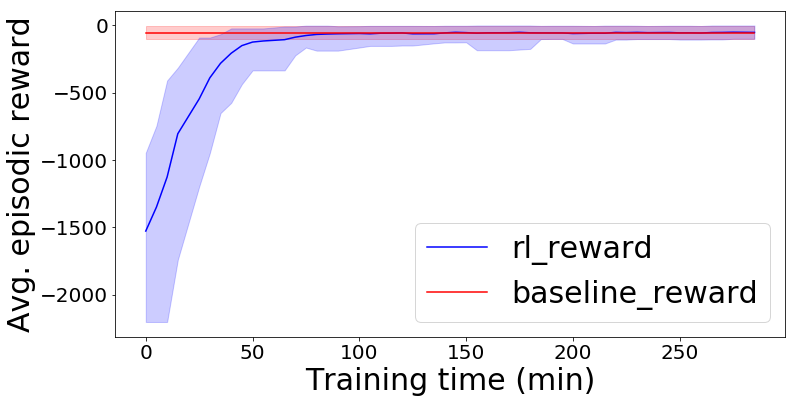
\includegraphics[width=1\linewidth]{images/bin_packing_rl_vs_baseline_bounded_waste_binsize_100.png}
%	\caption{RL vs baseline for BW distribution}
%	\label{fig:bin_packing_BW_dist1}
%\end{figure}
%
%\begin{figure}[h!]
%	\centering
%	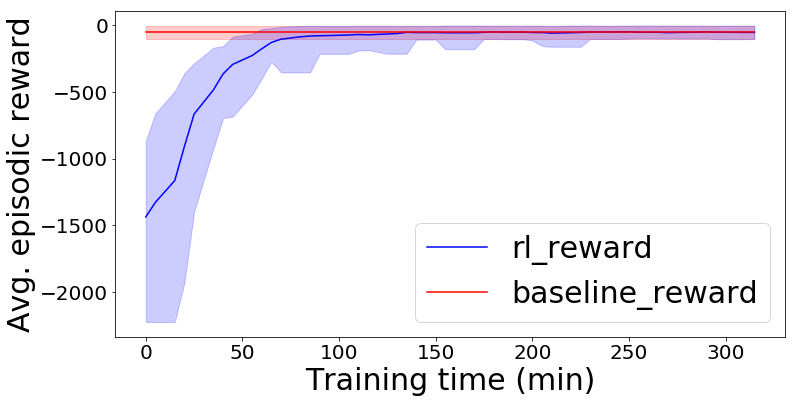
\includegraphics[width=1\linewidth]{images/bin_packing_rl_vs_baseline_perfect_pack_binsize_100.png}
%	\caption{RL vs baseline for PP distribution}
%	\label{fig:bin_packing_PP_dist1}
%\end{figure}
%
%\begin{figure}[h!]
%	\centering
%	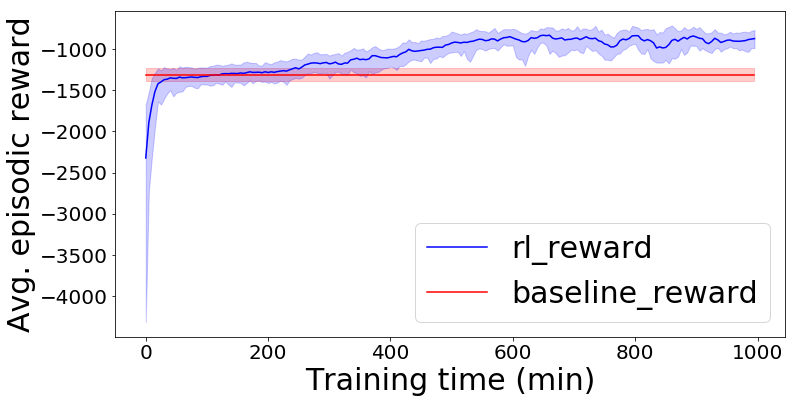
\includegraphics[width=1\linewidth]{images/bin_packing_rl_vs_baseline_linear_waste_binsize_100.png}
%	\caption{RL vs baseline for LW distribution}
%	\label{fig:bin_packing_LW_dist1}
%\end{figure}

\begin{figure*}
	\centering
	\begin{subfigure}[b]{0.33\textwidth}
		\centering
		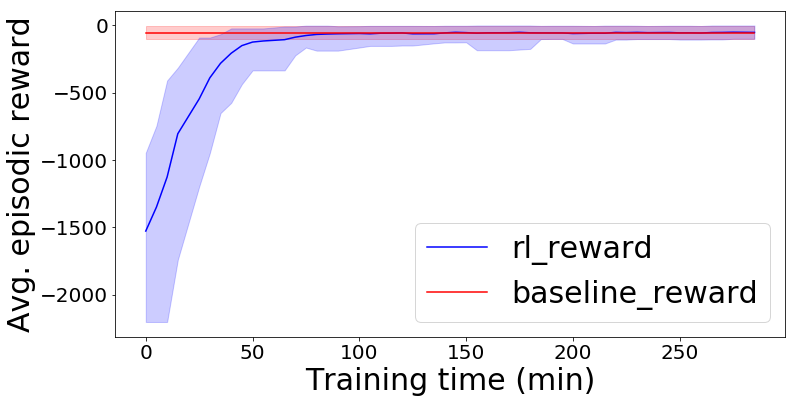
\includegraphics[width=\textwidth]{images/bin_packing_rl_vs_baseline_bounded_waste_binsize_100.png}
		\caption{RL vs baseline for BW distribution}
		\label{fig:bin_packing_BW_dist1}
	\end{subfigure}
	\hfill
	\begin{subfigure}[b]{0.33\textwidth}
		\centering
		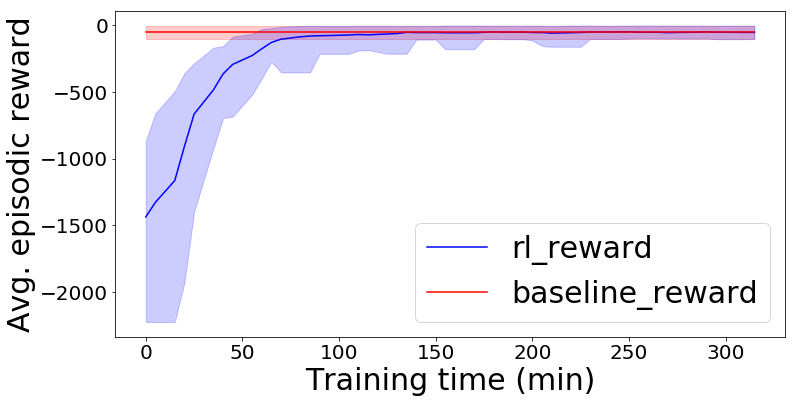
\includegraphics[width=\textwidth]{images/bin_packing_rl_vs_baseline_perfect_pack_binsize_100.png}
		\caption{RL vs baseline for PP distribution}
		\label{fig:bin_packing_PP_dist1}
	\end{subfigure}
	\hfill
	\begin{subfigure}[b]{0.33\textwidth}
		\centering
		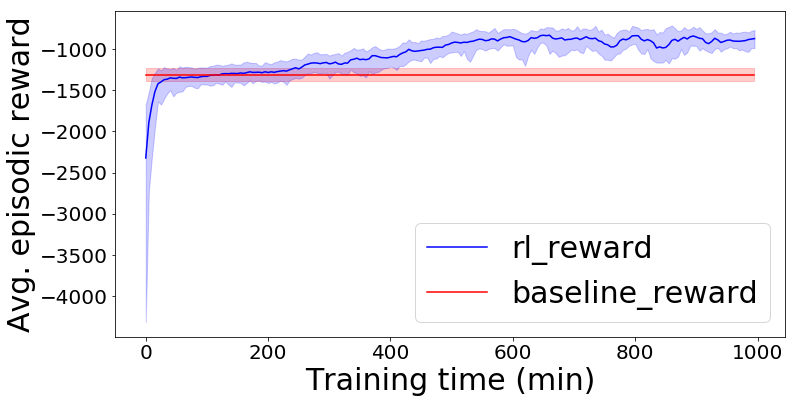
\includegraphics[width=\textwidth]{images/bin_packing_rl_vs_baseline_linear_waste_binsize_100.png}
		\caption{RL vs baseline for LW distribution}
		\label{fig:bin_packing_LW_dist1}
	\end{subfigure}
	\caption{Comparison of episodic rewards between RL and Best Fit baseline during training.}
	\label{fig:RLvsBF_binpacking}
		\vspace{-1em}
\end{figure*}


Figure \ref{fig:RLvsBF_binpacking} plots the reward function of the RL policy in training (blue) vs the Best Fit baseline (red) for bin size 100 and different item size distributions (BW, PP, and LW) as a function of training time (measured in minutes). The solid lines represent the mean reward of each policy, and the shaded bands represent the min/max rewards. By the end of training, RL either matches or outperforms the baseline policy for all three item size distributions. In particular, the reward gap between RL and baseline is the largest for LW distribution (which is expected, as both BF and SS are known to be suboptimal for LW distribution). %The min reward of RL sometimes falls below that of SS as RL tries to explore different actions in training.

%\textcolor{red}{REDO Table 2}

In Table \ref{table:bin_packing_RL_baseline_comp}, we inspect numerically the trained RL policy vs. baseline for bin size 100.  Note that the exploration is turned off for the trained RL policy.  Supporting what we observed in the initial figures, this table shows the final RL policy outperformes or matches the baseline for each distribution.
%\begin{table}[h!]
%	\centering
%	\begin{tabular}{ |c|c|c|c| } 
%		\hline
%		Algorithm & Perfect Pack & Bounded Waste & Linear Waste \\ 
%		\hline
%		\multirow{3}{4em}{RL}  & Bounded Waste & -53.86 & 26.4  \\ 
%		& Perfectly Packable & -50.5  & 28.3 \\
%		& Linear Waste  &   -880.2 &   43 \\
%		\hline	
%		\multirow{3}{4em}{SS} & Bounded Waste & -55.5 & 28.4 \\ 
%		& Perfectly Packable & -55.54  & 28.4  \\ 
%		& Linear Waste &  -2091 & 92 \\ 
%		\hline
%		\multirow{3}{4em}{BF} & Bounded Waste & -51.4  & 28.9  \\ 
%		& Perfectly Packable & -52.01  & 29.5\\ 
%		& Linear Waste &  -1314 & 53 \\ 
%		\hline
%	\end{tabular}
%	\caption{Comparison between RL and baseline.}
%	\label{table:bin_packing_RL_baseline_comp}
%\end{table}

We test generalization of the RL policy by evaluating the trained policy with a different item distribution than the one it was trained on. For PP and BW distributions, the trained policy mutually translate well. Both the PP and BW policies perform as well as the baseline solutions for the LW distribution. The policy trained on the LW distribution generalizes reasonably well but does not do as well as the baseline solutions in the BW and PP distributions. We did observe overfitting if we pick model iterations from much later in training. We leave study of overfitting and generalization across distributions as future work. A note on scaling: the training time for bin size 100 compared to bin size 9 is about 3x, 4x and 10x more for PP, BW and LW respectively. Appendix \ref{appendix:bin_size_9} has the bin size 9 results.
%The full results of bin size 9 experiments is given in Appendix \ref{appendix:bin_size_9}.

\begin{table}[h!]
	\resizebox{\columnwidth}{!}
	{%
		\begin{tabular}{|c|cc|cc|cc|}
			\hline
			\multicolumn{1}{|l|}{\multirow{2}{*}{Algorithm}}  & \multicolumn{2}{c|}{Perfect Pack} & \multicolumn{2}{c|}{Bounded Waste}	& \multicolumn{2}{c|}{Linear Waste} \\
			\multicolumn{1}{|l|}{} 											&   $\mu$            &        $\sigma$		& 	$\mu$    			& 	$\sigma$     		 &     $\mu$        &      $\sigma$          \\ \hline
			RL with PP  										  & -49.0     		   &          29.5        	&  	-48.0 	  			  &   29.5	 				 &     -1358       &      44.2     \\ \hline
			RL with BW  									  & -47.6     		   &          29.3        	&  	-53.9 	  			  &   26.4	 				 &     -1368       &      48.0     \\ \hline
			RL with LW 										 &  -258.6     		  &         69.3           &  	-143.9 	  			&   84.9	 			   &     -880.2      &      43     \\ \hline
			SS  											   &  -56.54     	    &         28.9           &    -56.61 	  			&   30.2	 			   &     -2091      &      92     \\ \hline
			Best Fit  															  &  -52.01     	   &          29.5           &  	-51.4 	  			&   28.9	 			   &     -1314     &      53     \\ \hline
		\end{tabular}
	}
	\caption{RL and baseline solution comparison for bin packing. Mean and standard deviations are calculated across 100 episodes.}
	\label{table:bin_packing_RL_baseline_comp}
		\vspace{-1em}
\end{table}

Finally, we inspect the relative structure of the policies to ensure that RL is learning a sensible solution.  In particular, we plot the state variable values as a function of the number of steps in an episode. Intuitively, the integral of these plots represents the waste, which we want to minimize.  An optimal policy should show a (relatively) flat surface. We use bin size of 9 for this analysis for ease of manual inspection and study the linear waste distribution that highlights the difference between the Sum of Squares baseline and RL distinctly. From Figure \ref{fig:bin_packing_LW_dist}, we see that the baseline policy leaves more open bins at a lower fullness, whereas RL only leaves open bins at level 8 (which cannot be closed once they reach that level). For other distributions, the graphs for both the baseline and RL policy look similar to each other.

%For the PP distribution (Figure \ref{fig:bin_packing_PP_dist}), we see that RL converges to a structure very similar to the baseline, but again with a little more smoothness prior to bin-level 8.

%Finally, for the BW distribution (Figure \ref{fig:bin_packing_BW_dist}), RL is most impressive relative to the baseline, as RL avoids entirely the bin-level 8 trap and achieves a nearly perfectly flat surface. Together, these plots show that RL is learning a policy structure similar to what we expect from the baseline, but with some improvements toward optimality (especially in the BW case).

\begin{figure}[h!]
	\centering
	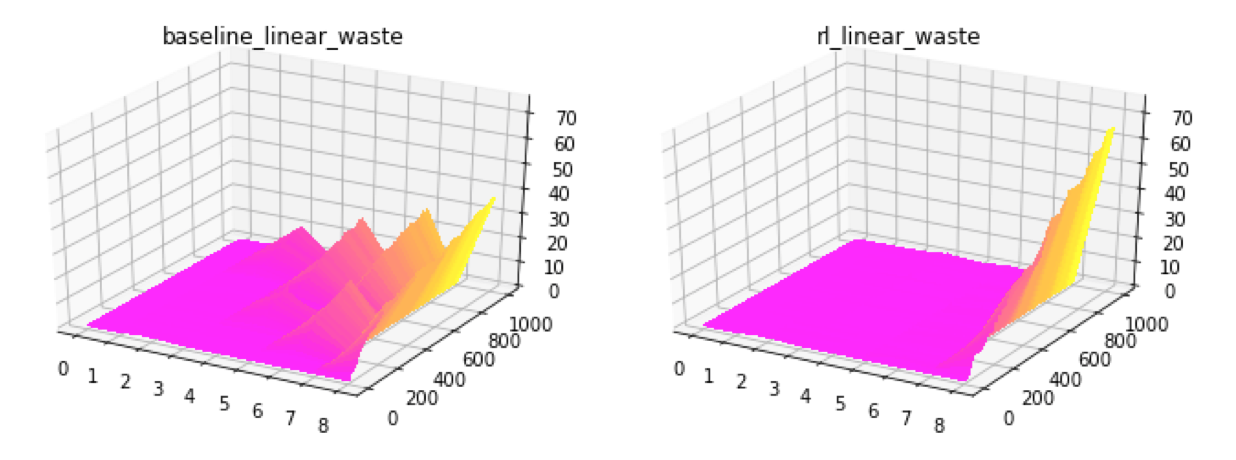
\includegraphics[width=1\linewidth]{images/linear_waste_sol.png}
	\caption{RL vs baseline solution for LW distribution}
	\label{fig:bin_packing_LW_dist}
		\vspace{-1em}
\end{figure}

%\begin{figure}[h!]
%	\centering
%	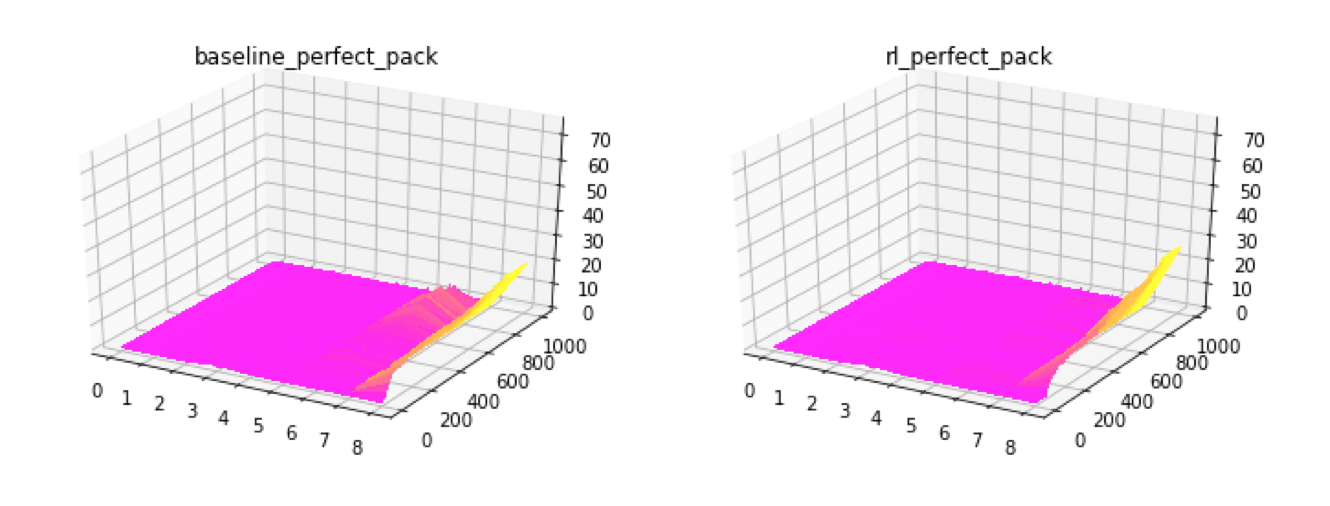
\includegraphics[width=1\linewidth]{images/perfect_packing_sol.png}
%	\caption{RL vs baseline solution for PP distribution}
%	\label{fig:bin_packing_PP_dist}
%\end{figure}
%
%\begin{figure}[h!]
%	\centering
%	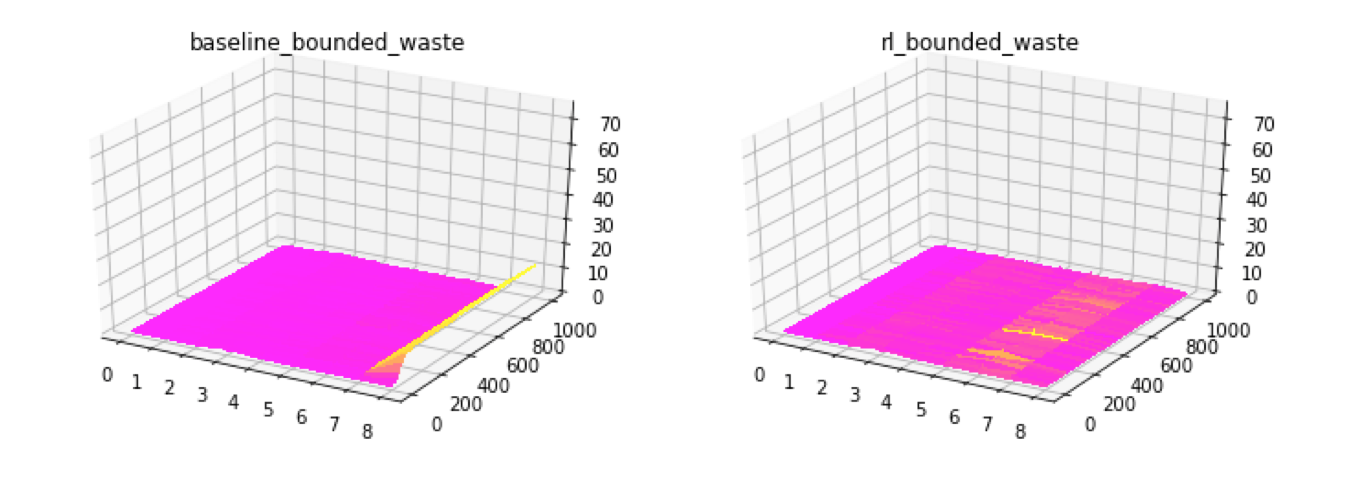
\includegraphics[width=1\linewidth]{images/bounded_waste_sol.png}
%	\caption{RL vs baseline solution for BW distribution}
%	\label{fig:bin_packing_BW_dist}
%\end{figure}

%Note that for all items size distributions, solution returned by RL uses many more bins at fullness level of 8 or 9 (recall that bin size is 9), whereas SS also uses more bins at lower fullness level compared to RL. 
%Below is an example of the frequency of bins of different fullness level for one run of RL vs baseline for each of the three size distributions:
\ifx
\begin{table}[h!]
	\centering
	\begin{tabular}{ |c|cc|cc|cc| } 
			\hline
Fullness Level&LW&&PP&&BW& \\
\hline
& RL&SS&RL&SS&RL&SS \\
\hline

2 & 0 & 1 & 0 & 0 & 0 & 0 \\
\hline
3 & 0 & 0 & 2 & 0 & 0 & 0 \\
\hline
4 & 0 & 9 & 0 & 1 & 0 & 0 \\
\hline
5 & 1 & 0 & 0 & 0 & 0 & 0 \\
\hline
6 & 0 & 16 & 0 & 9 & 0 & 2 \\
\hline
7 & 0 & 0 & 0 & 0 & 1 & 0 \\
\hline
8 & 78 & 27 & 19 & 18 & 0 & 10 \\
\hline
9 & 173 & 208 & 233 & 229 & 278 & 271 \\
\hline
Total Reward & -82 & -127 & -31 & -50 & -2 & -16 \\
		\hline
	\end{tabular}
	\caption{Comparison between RL and baseline solutions.}
	\label{table:bin_packing_RL_baseline_sol_comp}
\end{table}
\fi
\ifx
\begin{table}[h!]
	\centering
	\begin{tabular}{ |c|c|c| } 
		\hline
		Packing Type & RL & SS \\ 
		\hline
		2 & 0 & 1  \\ 
		\hline
		2,2 & 0 & 9 \\
		\hline
		2,3 & 1 & 0 \\
		\hline
		2,2,2 & 0 & 16 \\   
		\hline
		2,2,2,2 & 76 & 26 \\
		\hline
		2,3,3 & 2 & 1 \\
		\hline
		2,2,2,3 & 169 & 206 \\
		\hline
		3,3,3 & 4 & 2 \\
		\hline
		Total Reward & -82 &-127 \\
		\hline
	\end{tabular}
\end{table}

\begin{table}[h!]
	\centering
	\begin{tabular}{ |c|c|c| } 
		\hline
		Packing Type & RL & SS \\ 
		\hline
		3 & 2 & 0 \\
		\hline
		2,2 & 0 & 1 \\
		\hline
		2,2,2 & 0 & 9 \\   
		\hline
		3,3 & 0 & 0 \\
		\hline
		2,3,3 & 3 & 3 \\
		\hline
		2,2,2,2 & 16 & 15 \\
		\hline
		2,2,2,3 & 226  & 215 \\
		\hline
		3,3,3 & 7 & 14 \\
		\hline
		Total Reward & -31 &-50 \\
		\hline
	\end{tabular}
\end{table}

\begin{table}[h!]
	\centering
	\begin{tabular}{ |c|c|c| } 
		\hline
		Packing Type & RL & SS \\ 
		\hline
		2,2,2 & 0 & 1 \\   
		\hline
		3,3 & 0 & 1 \\
		\hline
		2,2,3 & 1 & 0 \\
		\hline
		2,3,3 & 0 & 10 \\
		\hline
		2,2,2,3 & 163 & 152 \\
		\hline
		3,3,3 & 115 & 119 \\
		\hline
		Total Reward & -2 &-16 \\
		\hline
	\end{tabular}
\end{table}
\fi



%!TEX root = or_benchmarks_paper.tex
\section{Multi-Period Newsvendor Problem with Lead Times}
\label{sec:newsvendor}

The Newsvendor problem (see e.g. \cite{zipkin2000foundations}) is a seminal problem in inventory management wherein we must decide on an ordering decision (how much of an item to purchase from a supplier) to cover a single period of uncertain demand. The objective is to trade-off the various costs incurred and revenues achieved during the period, usually consisting of sales revenue, purchasing and holding costs, loss of goodwill in the case of missed sales, and the terminal salvage value of unsold items.

In practice, decisions are rarely isolated to a single period, and they are repeatedly and periodically taken and thus have a downstream impact. This makes the problem non-trivial, as compared to the single-period Newsvendor which has a known solution when the demand distribution is known. Additionally, purchased units do not, in general, arrive quasi-instantaneously, but rather after a few periods of transit from the vendor to their final destination, known as the lead time. The presence of lead times further complicates the problem. The multi-period newsvendor problem with lead times under the lost-sales model, where customers leave if there is no stock to satisfy their demand, is known not to admit a simple solution such as an order-up-to policy (which maintains an inventory level, and orders up to that level whenever inventory levels fall).

% with a simple structure. Simple structures include an  as is the case in the absence of lead time or when a backlogging assumption is made.

Solving the multi-period newsvendor problem with lead times and lost sales is a notoriously difficult problem \citep{zipkin2008old}. It requires keeping track of orders placed in different periods, leading to what is known as the \emph{curse of dimensionality}, rendering any exact solution impractical even for small lead times of 2 and 3 periods, and outright infeasible at higher dimensions. As a result, the problem forms a good test-bed for RL algorithms given that the observation of rewards is delayed by the lead time and that it can be formulated as a Markov Decision Problem. Additionally, a number of heuristics have been developed for the lost sales problem, often based on order-up-to level policies for the equivalent model with backlogged demand. Comparisons in the performance of these two policies have been studied \cite{janakiraman2007comparison}, and it has been shown that order-up-to policies are asymptotically optimal and robust (in some sense) \cite{huh2009asymptotic,bijvank2014robustness}, thus making for good benchmark policies.

\subsection{Problem formulation}
We consider the stationary, single-product, multi-period dynamic inventory management problem with vendor lead time (VLT) and stochastic demand. Here, the VLT $l$  refers to the number of time steps between the placement  and receipt of an order. The demand $D$ is assumed to be stationary and Poisson distributed with mean $\mu$. Items are purchased at a cost $c$ and sold at a price $p$, and incur a penalty for lost sales $k$ for each unit of unmet demand while any unit left over at the end of a period incurs a holding cost $h$. A discount factor $\gamma$ is used.


The problem is formulated as a Markov Decision Process: 
\begin{description}[style=unboxed,leftmargin=0cm]
\item[State:] The state $S$ of the problem is given by
\begin{align*}
S=(p,c,h,k,\mu,x_0,\ldots,x_{l-1})
\end{align*}
where $x_0$ is the on-hand inventory, $x_1$ the units to be received one period hence, and so on.
\item[Action:] In each period the state of the system is observed and an action $A=q$ is taken, consisting of the size of the order placed and to arrive $l$ time periods later.
\item[Reward:] We first incur the purchasing cost corresponding to the procured units given the action $a$.
A realization $d$ of the demand $D$, which we recall is Poisson distributed with mean $\mu$, is then observed, and demand is satisfied as much as is possible given on-hand levels. Missed sales incur a loss of goodwill $k$ per unit, while leftover units incur a holding cost $h$:
\begin{align*}
R &= p\min(x_0,d) - c a - h (x_0 - d)^+ - k (d - x_0)^+.
\end{align*}
where $(x)^+=\max(x,0)$.
\item[Transition:] The state of the system $S$ is then updated to $S_+$ by moving all pipeline units downstream and incorporating the newly purchased units:
\begin{align*}
S_+ &= (p,c,h,k,\mu,(x_0 - d)^+ +x_1,x_2,\ldots,x_{l-1},a).
\end{align*}
\end{description}

\subsection{Related work}
Some recent work has started looking at the newsvendor problem using a data-centric approach \cite{rudin2014big} or a reinforcement learning approach \cite{oroojlooyjadid2016applying}. These have so far still remained focused on the single period problem and often trying to learn some of the inputs, such as demand. Few other papers have considered Reinforcement Learning in the context of inventory management, such as \cite{gijsbrechts2018can} where a dual sourcing problem is tackled using RL.

\subsection{Baseline solution} 

As noted in Section \ref{sec:newsvendor}, it is impractical or even infeasible to solve the problem exactly to get a baseline. However, it is possible to use heuristics that provide good approximations to the optimal solution. In particular, a way to tackle the problem is to approximate it by its backlogging counterpart, for which a closed form solution of the optimal policy exists in the form of an order-up-to policy characterized by the following critical ratio:
\begin{align*}
CR = \frac{p-\gamma c + k}{p-\gamma c + k + h}.
\end{align*}
As a result, letting $z^* = F_l^{-1}(CR)$, where $F_l$ is the cumulative distribution  function of the $l$ period demand, the policy is given by:
\begin{align*}
a&= \left(z^* - \sum_{i=0}^{l-1} x_i\right)^+.
\end{align*}


\subsection{RL solution} 


We used a Proximal Policy Optimization algorithms (PPO) \cite{schulman2017proximal} as implemented in the RLLib package \cite{liang2017rllib}, where the policy is represented by a neural network. We used a neural network of size (256,256) and the hyperparameters presented in Appendix \ref{appendix:newsvendor_hp}.


\subsection{Results}

We present the results obtained using a VLT of 5. The economic parameters were chosen so that $p,c\in[0,100]$, $h\in[0,5]$ and $k\in[0,10]$, while the demand mean $\mu$ was such that $\mu\in[0,200]$.

In the course of our experiments we saw that how we sampled the initial state and item characteristics is critical. We modified the sampling scheme so as to sample ``interesting" states and avoid trivial or misleading initial configurations. For example, it should be easily learned that nonprofitable items (including the penalty for lost sale) should not be purchased, but this is not really indicative of a good performance since in practice such items would not be part of inventory. Similarly, high initial inventory levels would not lead to any purchase either because inventory can simply be drained over long periods of time, resulting in a trivial decision that results in a high reward that would unfairly favor the perceived quality of the RL solution. 

As a result, the sampling was performed as follows: $p\sim U[0,100]$, $c\sim U[0,p]$, $h\sim U[0,\min(c, 5)]$, $k\sim U[0,10]$ and $\mu\sim U[0,200]$ for the economic and demand parameters; where $U[a,b]$ denotes a uniformly random variable between $a$ and $b$.  The initial state was simply set to be $\mathbf{0}$.
%The initial state was similarly sampled so as to be in a region where actions are meaningful: $x_0\sim U[0,l\mu]$ and $x_{i} \sim U[0,l\mu - \sum_{j=0}^{i-1} x_j]$ for $i=1,\ldots,l-1$; where $U[a,b]$ denotes a uniformly random variable between $a$ and $b$.

%Figure~\ref{fig:newsvendor_PPO} compares the results obtained by the RL algorithm to the baseline. As noted earlier, the results do not give full credit to the RL approach in part because its reward function incorporates a penalty term to guide the policies towards the feasible region, which artificially decreases its perceived performance. Ongoing experiments are more promising and will be reported on in future work.

Figure~\ref{fig:newsvendor_PPO} compares the results obtained by the RL algorithm to the baseline. We observe that the RL solution was nearing the benchmark when the experiment was stopped.


\begin{figure}
\centering
        %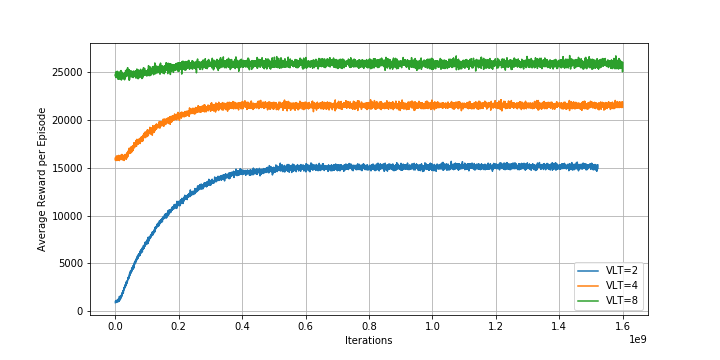
\includegraphics[width=0.5\textwidth]{images/newsvendor_PPO_big_minibatch_mlp_20_10.png}
        %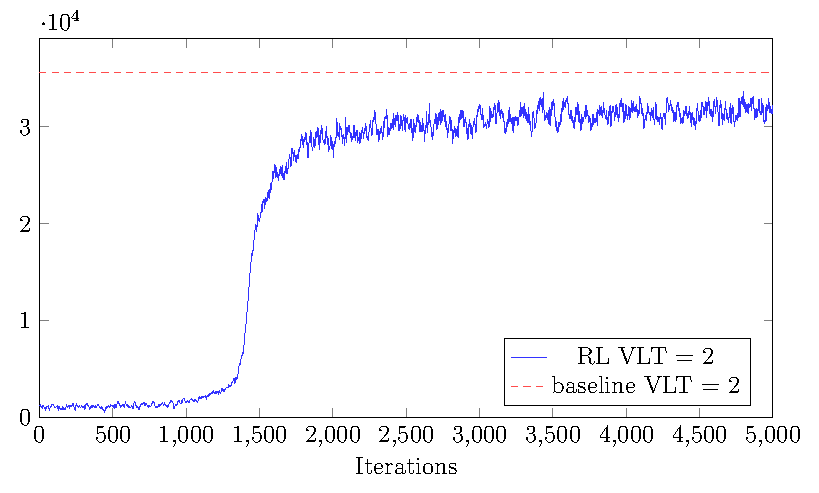
\includegraphics[width=0.45\textwidth]{images/newsvendor_l_2_ppo.pdf}
        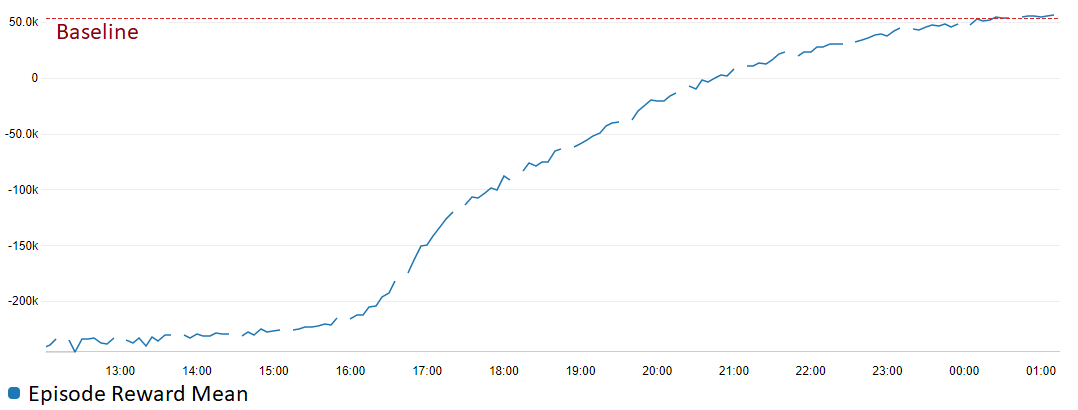
\includegraphics[width=0.45\textwidth]{images/newsvendor_edit.png}
    \caption{RL solution reward in the newsvendor problem.}
    \label{fig:newsvendor_PPO}
    	\vspace{-1em}
\end{figure}

While solving this problem numerically is intractable, the optimal inventory policy structures are well known. It is thus of interest to check whether their properties are being learned by the RL algorithm. Given the dimension of the problem, we cannot observe the entire policy, but can investigate slices thereof. We thus fix price, cost, holding cost, penalty for lost sale and mean demand to 50, 25, 0.5, 5 and 100, respectively, and plot the optimal policy in the space $(0,0,x_2,x_3,0)$ in Figure~\ref{fig:newsvendor_policy}. The figure shows contour curves of the buying quantity as a function of the inventory state. We observe that the algorithm is slowly learning the policy structure and we can start to observe monotonicity of the policy along most directions.

\begin{figure}[htbp]
\centering
        %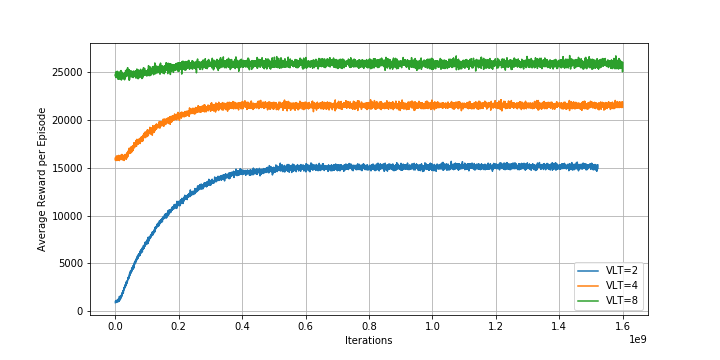
\includegraphics[width=0.5\textwidth]{images/newsvendor_PPO_big_minibatch_mlp_20_10.png}
        %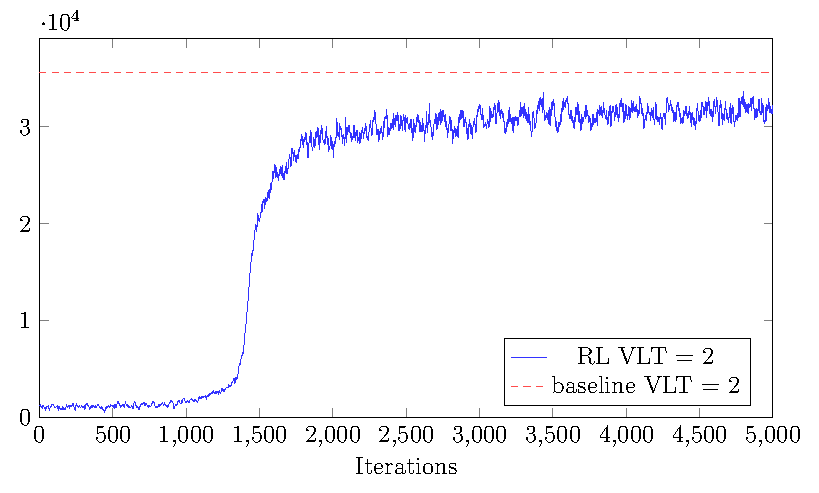
\includegraphics[width=0.45\textwidth]{images/newsvendor_l_2_ppo.pdf}
        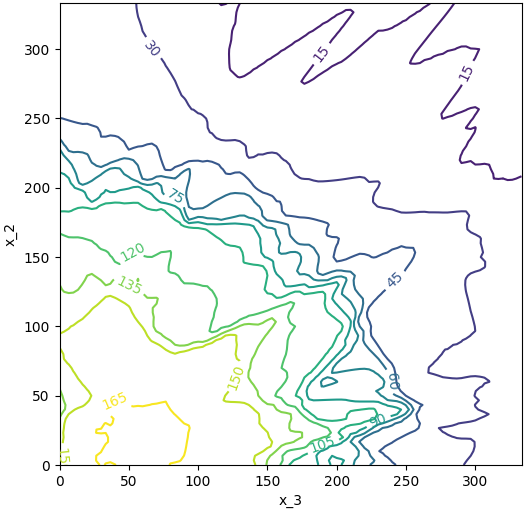
\includegraphics[width=0.4\textwidth]{images/newsvendor_policy.png}
    \caption{Slice of the learnt policy for the multi-period newsvendor.}
    \label{fig:newsvendor_policy}
    	\vspace{-1em}
\end{figure}


\section{Vehicle Routing Problem}
\label{sec_vrp_intro}

In the traveling salesman problem (TSP), we find the shortest route that visits each node in a graph exactly once and returns to the starting node. TSP is one of the most widely studied problems in combinatorial optimization both due to its NP-hard nature and as well as its wide variety of practical applications. The vehicle routing problem (VRP) is a generalization of TSP where one or more vehicles are expected to visit the nodes in a graph, usually to satisfy customer demand. VRP is also a well studied topic and has very important applications, especially in supply chain and logistics. These real-life applications lead to many variants of VRP with different constraints, such as  capacitated vehicles, pickups and deliveries on the route, time windows associated with each pickup and delivery etc. 

An important extension of VRP is where some of the information about the graph is revealed over time, such as demand at each node and travel time. This class of VRP is called dynamic VRP (DVRP, also known as real-time or online VRP). Stochastic VRP (SVRP) is where one or more problem parameters are stochastic with some known probability distributions (as opposed to arbitrary or adversarial distributions). In many real-life applications, the relevant VRP is both stochastic and dynamic (SDVRP), which is also focus of this work. We formulate a variant of SVRP and compare solution approaches from the Operations Research (OR) and Reinforcement Learning (RL) literature.

\subsection{Problem Formulation}
\label{sec_vrp_pf}

We consider a decentralized version of the VRP. Consider a delivery driver using a phone app, orders arrive on the app in a dynamic manner. Each order has a delivery charge known to the driver at the time of order creation, and it is assigned to a location in the city. "City" here means the whole Euclidean space in which the VRP problem lives. The city consists of mutually exclusive zones ($num\_zones = 4$) that generate orders at different rates ($order\_probs\_per\_zone = (0.5, 0.3, 0.1, 0.1)$) and with rewards according to truncated normal distribution with different ranges ($order\_reward\_max = (12, 8, 5, 3), order\_reward\_min = (8, 5, 2, 1)$). The orders have a delivery time limit ($order\_promise = 60$), the timer starts with the order creation and is same for all orders. The driver has to accept an order and pick up the package from a given location prior to delivery. Orders that are not accepted disappear probabilistically ($order\_timeout\_prob = 0.15$) when other drivers accept the orders. The vehicle has a capacity limit ($driver\_capacity = 4$), but the driver can accept unlimited orders and plan their route accordingly.  
%there is no limit on the number of orders that are accepted (but not picked up or delivered) by the driver at the same time. Finally, 
Each time step and unit distance travelled adds a fixed cost $(penalty\_per\_timestep = 0.1, \ penalty\_per\_move = 0.1)$, and the episode length is $1000$. The driver's goal is to maximize the total net reward. Our formulation is known as stochastic and dynamic capacitated vehicle routing problem with pickup and delivery, time windows and service guarantee. % (SDPDPTW with service guarantee).

\subsection{Related Work} \label{sec_vrp_related_work}
There is a substantial literature on VRP~\cite{EKSIOGLU20091472}. The closest VRP variant to the problem considered in this paper is the Pickup and Delivery Problem with Time Windows (PDPTW) \cite{Cordeau2008}, which has some additional complexities over vanilla VRP. Due to such complexities, there are fewer exact solution approaches \cite{LuDessouky2004,MAHMOUDI201619}, and a majority of the literature focuses on heuristics. When the problem is also stochastic and dynamic, exact solution methods become intractable except for very specific problem settings. In such cases, anticipatory algorithms that simulate sample future scenarios and merge solutions to those samples are a common choice \cite{BERBEGLIA20108, Berhan2014, Ulrike2016, Ghiani2012}.

Reinforcement Learning (RL) methods have been successfully used for solving the Traveling Salesman Probelm (TSP). \citet{bello2016neural} employ a pointer network \cite{vinyals2015pointer} to optimize the policy, and train an actor-critic algorithm with the negative tour length as the reward signal. \citet{khalil2017learning} develop a single model based on graph embeddings. They use the DQN algorithm to train a greedy policy and graph embedding network simultaneously.  For VRP, \citet{kool2018attention} utilize the Transformer architecture \cite{vaswani2017attention} to develop a model fully based on attention layers. Their proposed model is trained by policy gradients with a greedy baseline, and evaluated on both standard Capacitated VRP (CVRP) and Split Deliverry VRP (SDVRP). \citet{nazari2018reinforcement} further improve the algorithm using embedded inputs and allow the customers and their demands to be stochastic. Besides, \citet{lin2018efficient} propose a contextual multi-agent reinforcement learning framework for fleet management, and use a simulator that mimics the process of online order generation/asignment in real world.

%While traditional VRP focuses on minimizing the tour length, we extend this criterion to integrate order values to learn if the agent can prioritize profitable orders. We consider a more complex environment with multiple zones with different order distributions. In addition, we have time limits for service guarantee. We believe these changes translate better to practical use cases. We also show that a simple 2-layer neural network suffices to learn good policies even in such complex environments.

\subsection{Baseline Algorithm}
We modify the classical three-index Mixed Integer Programming (MIP) formulation \cite{LuDessouky2004,RopkeCordeau2009, FURTADO2017334}. This deterministic MIP is solved for the available orders in the environment. It is further resolved when a new order arrives, if one of the existing orders expires or, when all of the actions are executed. When we solve the MIP, orders already accepted or in transit are modeled as starting conditions. The details of our MIP model is given in Appendix \ref{appendix:vrp_mip}. We leave anticipatory models to future work (see Section \ref{sec_vrp_related_work}).

%Note that when the MIP is solved, some of the orders could have been accepted due to the previous solution and some of the orders could be already in transit. Our version of the model (as opposed to the classical formulation in literature) enforces such starting conditions. 

\ifx
\subsubsection*{Sets}
\begin{vardefs*}
V & Current vehicle location, $V=\{0\}$ \\
P & Pickup nodes (copies of the restaurant nodes, associated with the orders that are not in transit)  \\
D & Delivery nodes representing the orders that are not in transit, $D = \{j | j= i + n, i \in P, n=|P| \}$  \\
A & Nodes representing the orders that are accepted by the driver; $A \subset D$ \\
T & Delivery nodes representing the orders that are in transit  \\
R & Nodes representing the restaurants, used for final return) \\
N & Set of all nodes in the graph, $N = V \cup P \cup D  \cup T \cup R $\\
E & Set of all edges, $E=\{(i, j),  \forall i, j \in N\}$
\end{vardefs*}


\subsubsection*{Decision variables}
\begin{vardefs*}
 x_{ij} & Binary variable, 1 if the vehicle uses the arc from node $i$ to $j$, 0 otherwise; $i, j \in N$ \\
y_{i}  & Binary variable, 1 if the order $i$ is accepted, 0 otherwise; $i \in P$\\
Q_{i} & Auxiliary variable to track the capacity usage as of node  $i$; $i \in N$ \\ 
B_{i} & Auxiliary variable to track the time as of node  $i$; $i \in N$
\end{vardefs*}

\subsubsection*{Parameters}
\begin{vardefs*}
n & Number of orders available to pick up, $n = |P|$ \\ 
c_{ij} & Symmetric Manhattan distance (in miles) matrix between node $i$ and $j$, $(i, j) \in E$ \\
q_i & Supply (demand) at node $i$, $q_0 = |T|; q_i = 1, \forall i \in P;  q_i = -1, \forall i \in D \cup T; q_i = 0 \in R$  \\ 
l_i & Remaining time to deliver order $i$, $i \in D \cup T$ \\ 
m & Travel cost per mile \\
r_i & Revenue for order associated with pick up node $i$, $i \in P$  \\
U & Vehicle capacity  \\
M & A very big number  \\ 
t & Time to travel one mile  \\
d & A constant positive service time spent on accept, pickup, delivery
\end{vardefs*}

\subsubsection*{Model}
\begin{equation}
\begin{array}{rrclcl}
& \max_{x, y, Q, B} & \multicolumn{3}{l}{ \sum_{i \in P} r_i y_i - m \sum_{(i,j) \in E} c_{ij} x_{ij}  } \\  
& \textrm{s.t.} \qquad  \sum_{j \in N} x_{ij}   &=& y_i & \forall i \in P \\   %leave
& \sum_{j \in N} x_{ij} - \sum_{j \in N} x_{i+n,j}  & = & 0 & \forall i \in P  \\     %pickup
& y_i & =& 1 & \forall i \in A \\  % accepted
& \sum_{j \in N} x_{ij}   &=& 1 & \forall i \in V \cup T \\  % start and  in-transit
& \sum_{i \in N \setminus R } \sum_{j \in R }  x_{ij}   &=& 1  &\\     %end 
& \sum_{j \in N \setminus R } x_{ji} - \sum_{j \in N} x_{ij}  & = & 0 & \forall i \in P \cup D \cup T  \\     %flow
& Q_i + q_j - M (1-x_{ij} ) &\leq& Q_j & \forall i,j \in N \\  %captrack
& \max{(0, q_i)}    &\leq& Q_i & \forall i \in N \\  %cap_lb
& \min{(U, U+q_i)}    &\geq& Q_i & \forall i \in N \\  %cap_ub
& B_i + d + c_{ij} t -  M (1-x_{ij} )  &\leq& B_j   & \forall i,j \in N \\  %time_track , *\mathcal{1}\{ i \notin V  \}
& B_i +  c_{i, i+n} t -  M (1- y_i )  &\leq& B_{i+n}  & \forall i \in P \\ %precedence
&  d \sum_{i \in P \setminus A}  y_i  & = & B_0  \\ %timetoaccept
& B_i  &\leq& l_i  & \forall i \in D \cup T \\ %precedence
& x_{ij}, y_i &\in& \{0, 1\} & \forall i,j \in N  \\ 
\end{array}
\end{equation}
\fi

\begin{figure*}[h!]
	\centering
	\begin{subfigure}[b]{0.45\textwidth}
		\centering
		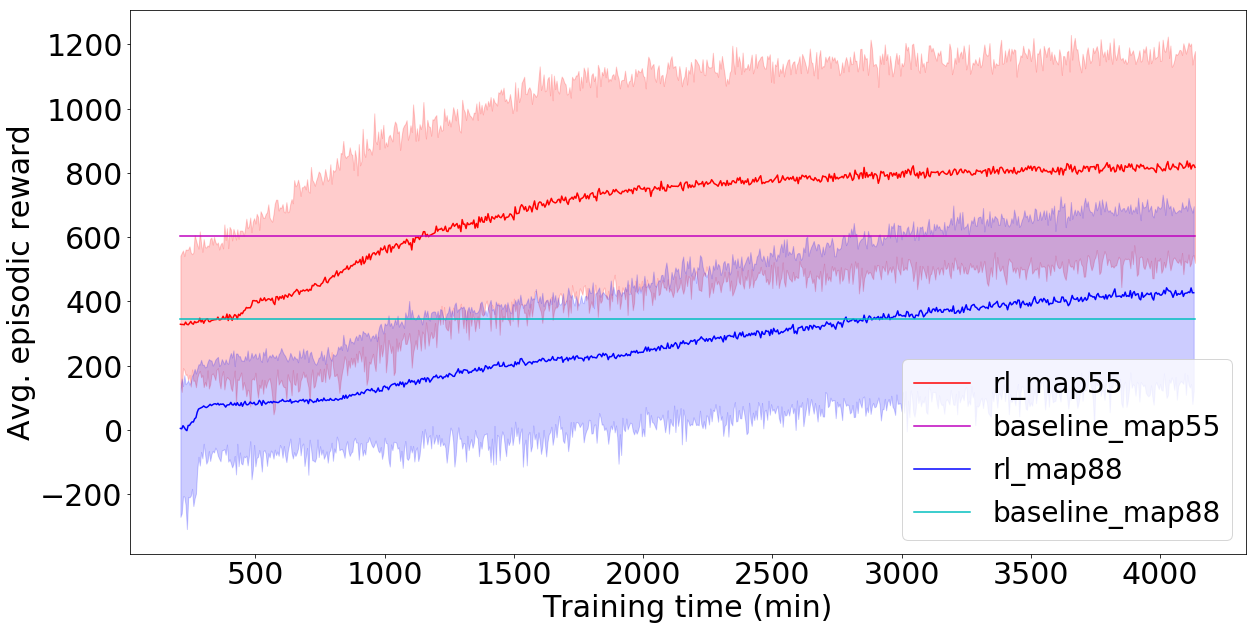
\includegraphics[width=1\linewidth]{vrp_images/vrp_mapsize.png}
		\caption{RL vs baseline solution for VRP with 3 pick-up locations, 5 orders and map sizes $5 \times 5$ and $8 \times 8$ }
		\label{fig:vrp_mapsize}
	\end{subfigure}
	\hspace{2em}
	\begin{subfigure}[b]{0.45\textwidth}
		\centering
		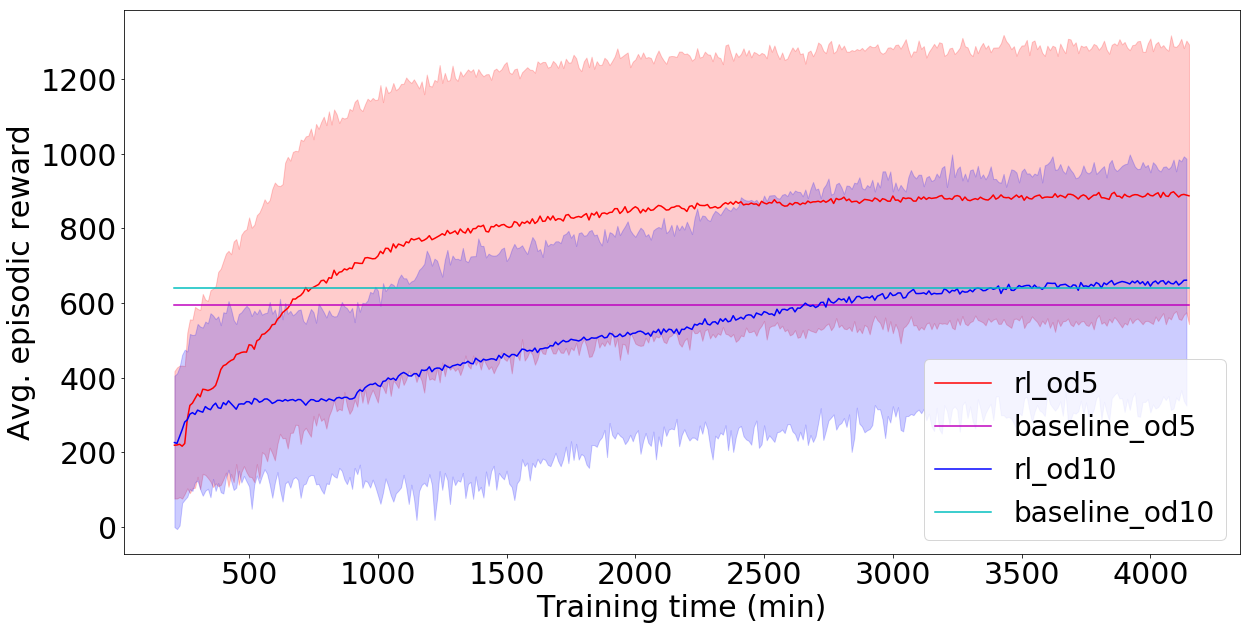
\includegraphics[width=1\linewidth]{vrp_images/vrp_ordernumber.png}
		\caption{RL vs baseline solution for VRP with 2 pick-up locations, map $5 \times 5$, and number of orders 5 and 10. }
		\label{fig:vrp_ordernumber}
	\end{subfigure}
\label{fig:vrp}
\caption{RL vs baseline during policy training process.}
	\vspace{-1em}
\end{figure*}

\subsection{Reinforcement Learning Algorithm}
\label{subsec:vrp_rl}
%We consider a Markov Decision Process (MDP) formulation to tackle this problem and cast the optimal routing path as a sequence of actions that an agent takes. 
\begin{description}[style=unboxed,leftmargin=0cm]
	\item[State:] 
	We include pickup location $\mathbf{p}_t$, driver info $\mathbf{d}_t$, and order info $\mathbf{o}_t$. Driver info contains the driver's position $\mathbf{h}_t$ and the capacity left $c_t$. Order info contains the orders' location $\mathbf{l}_t$, status $\mathbf{w}_t$ (open, accepted, picked up or delivered), the time elapsed since each order's generation $\mathbf{e}_t$ and the corresponding dollar value $\mathbf{v}_t$.  Thus, the state is  $S_t = (\mathbf{p}_t, \mathbf{d}_t, \mathbf{o}_t)$, in which $\mathbf{d}_t = (\mathbf{h}_t, c_t)$, $\mathbf{o}_t = (\mathbf{l}_t, \mathbf{w}_t, \mathbf{e}_t, \mathbf{v}_t)$.
	\item[Action] 
	The agent chooses an action $A_t$ from five options -- accept an order, pick up an accepted order, go to a customer's node for delivery, head to a specific pickup location, or wait and stay unmoved. 
	\item[Reward:] The reward $R_t$ is the total value of all delivered orders $\mathbf{f}_t$ minus the cost $\mathbf{q}$. $\mathbf{f}_t$ is divided into $3$ equal parts for reward shaping: when the order gets accepted, picked up, and delivered respectively. Thus we have:
	\begin{equation*}
			R_t = \frac{1}{3}\Big(\mathbbm{1}_{accepted} + \mathbbm{1}_{picked-up} + \mathbbm{1}_{delievered} \Big) \mathbf{f}_t - \mathbf{q}_t,
	\end{equation*}
	where $\mathbf{q}_t = (q_{time} + q_{move} + q_{failure})$. $q_{time}$ is the time cost, $q_{move}$ is the moving cost (per time step). $q_{failure}$ is a large penalty ($order\_miss\_penalty = 50$) if the agent accepts an order but fails to deliver within the promised time. 
	
\end{description}

The vehicle's capacity remains unchanged if an order is accepted but not picked up. In effect, this grants the agent the flexibility to accept more orders than its capacity, which can be picked up later when space allows. The action of heading to a specific pickup location enables the agent to learn to stay near popular pick up locations. % From a practical perspective, in a case where the majority of the customer orders come from a popular pick-up location, the agent may stay nearby even when there are currently no orders.

%The reward shaping also comes from a practical consideration. In essence, the order value is divided into $3$ parts to encourage order acceptance as well as pick-up, whereas the large penalty $q_{failsure}$ is imposed to prevent the agent from only accepting orders without successful deliveries. This way, we expect the learned policy to be capable of not only making full use of its capacity but also avoiding unsuccessful deliveries. 

We impose action masking during the policy training. The agent cannot perform the following invalid actions: \textit{(i)} pick up an order when its remaining capacity is $0$; \textit{(ii)} pick up an order that is not yet accepted; \textit{(iii)} deliver an order that is not yet picked up. 

To train the policy, we apply the APE-X \cite{horgan2018distributed} DQN algorithm due to its ability to scale by generating more experience replays and picking from them in a distributed prioritized fashion \footnote{We also applied PPO with default hyperparameters provided in RLLib. The reward increased much slower than that of APEX-DQN and was not able to beat baseline after 1-day training.}. We feed the input into a two-layer neural network with 512 hidden units each to compute the Q values. Appendix \ref{appendix:vrp_hp} lists the hyperparameters we use.

\subsection{Results}
For multiple problem scales determined by map size ($map\_size \in \{5 \times 5, 8 \times 8\}$), maximum number of orders ($order \in \{5, 10\}$) and number of pick-up location ($n \in \{2, 3\}$), we conduct experiments to compare the behavior of RL and the MIP baseline solutions. All experiments are conducted in Amazon EC2, where we use \texttt{p3.2xlarge} instances (1 GPU, 16 GPU memory, 8 vCPUs, 61  GB memory and up tp 10 Gbps link). We examine the trained RL policy's ability to generalize to different order distributions. The hyperparameters used for algorithm training are taken from RLLib examples without fine-tuning (Table \ref{table:vrp_hyperparam}). Overall, the RL approach outperforms the baseline across different instance sizes, and generalizes well for unseen order patterns. 

Figure \ref{fig:vrp_mapsize}-\ref{fig:vrp_ordernumber} compares the episodic rewards for the RL policy and the baseline algorithm during training. The shaded band around the mean line shows the minimum and maximum rewards. For readability, the graphs are clipped to skip the initial $3.5$ hours of training as the rewards are highly negative and skew the Y-axis scale. With larger map size or higher order number, the training time required for the agent to achieve rewards equivalent to baseline is higher. This is expected as both the observation and action space increase, the agent requires more exploration to converge to a reasonable policy. Even after three days of training, the rewards for larger instances keep growing gradually. The agent slowly learns to fully utilize the vehicle capacity. Over time, the agent also learns to reject (not accept) orders which are likely to incur penalty. %With more training the RL agent has potential to achieve even higher rewards.

As the agent is trained longer, there is potential for the policy to overfit. In order to test this issue, we train another policy with a shifted hot order-zone distribution ($(0.1, 0.5, 0.3, 0.1)$), and evaluate against the baseline results both using the original order-zone distribution ($(0.5, 0.3, 0.1, 0.1)$). Table \ref{table:vrp_baseline_comp} summarizes the evaluation results. It is observed that the policy is able to outperform the baseline consistently during evaluation phase.
 %The reward during training is lower than that of the baseline, indicating the change we made results in a more difficult senario. However, the policy is able to outperform the baseline consistently during evaluation phase. %In future, we would like to test the agent robustness further by varying the per order rewards and number of zones in the map. 

We also present the rewards with and without the order miss penalty $q_{failure}$ to further understand the agent's behavior about order delivery misses. The reward values are close for problems with less number of pick up locations and fewer orders. As the number of pick-up locations become larger, the gap between the rewards increases. One explanation is the agent cannot multiplex order deliveries from different pick-up locations and the likelihood of missing the order delivery increases. This behavior is also seen if the number of orders is higher. Even though the RL agent reward is better than the baseline, there is still scope for improvement by reducing the number of order delivery misses.

\begin{table}[h!]
	\resizebox{\columnwidth}{!}{%
		\begin{tabular}{|c|cc|c|}
			\hline
			\multicolumn{1}{|l|}{\multirow{2}{*}{Problem Instance}}                          & \multicolumn{2}{|c|}{RL Evaluation Reward}                                                                               & \multirow{2}{*}{MIP Reward} \\
			\multicolumn{1}{|l|}{}                                                                               & \multicolumn{1}{l}{Without $q_{failure}$ }                                 & \multicolumn{1}{l|}{With $q_{failure}$ }                             &                             \\ \hline
			\begin{tabular}[c]{@{}c}5 by 5 map, 5 orders\\ 2 pick-up locations \end{tabular}                    & \begin{tabular}[c]{@{}c@{}}854.45 \\ (136.03)\end{tabular} & \begin{tabular}[c]{@{}c@{}}838.30 \\ (154.12)\end{tabular} & 595.91                      \\ \hline
			\begin{tabular}[c]{@{}c}5 by 5 map, 5 orders\\ 3 pick-up locations\end{tabular}  & \begin{tabular}[c]{@{}c@{}}754.27 \\ (116.48)\end{tabular} & \begin{tabular}[c]{@{}c@{}}730.40 \\ (132.75)\end{tabular} & 642.62                      \\ \hline
			\begin{tabular}[c]{@{}c}5 by 5 map, 10 orders\\ 2 pick-up locations \end{tabular}               & \begin{tabular}[c]{@{}c@{}}774.63 \\ (143.34)\end{tabular} & \begin{tabular}[c]{@{}c@{}}692.34\\ (200.65)\end{tabular}  & 640.01                      \\ \hline
			\begin{tabular}[c]{@{}c}8 by 8 map, 5 orders\\ 2 pick-up locations\end{tabular}                      & \begin{tabular}[c]{@{}c@{}}548.53 \\ (107.40)\end{tabular} & \begin{tabular}[c]{@{}c@{}}536.55 \\ (112.33)\end{tabular} & 410.58                      \\ \hline
			\begin{tabular}[c]{@{}c}8 by 8 map, 5 orders\\ 3 pick-up locations \end{tabular}                          & \begin{tabular}[c]{@{}c@{}}429.20 \\ (102.37)\end{tabular} & \begin{tabular}[c]{@{}c@{}}373.7 \\ (129.98)\end{tabular}  & 246.25                      \\ \hline
		\end{tabular}
	}
	\caption{RL and baseline solution comparison for VRP. Values in the brackets are standard deviations and mean reward is calculated using 50 episodes.}
	\label{table:vrp_baseline_comp}
		\vspace{-1em}
\end{table}

%\begin{table}[h!]
%	\resizebox{\columnwidth}{!}{%
%	\begin{tabular}{|c|c|cc|c|}
%		\hline
%		\multicolumn{1}{|l|}{\multirow{2}{*}{Problem Instance}}                              & \multirow{2}{*}{RL Training Reward} & \multicolumn{2}{c|}{RL Evaluation Reward}                                                                               & \multirow{2}{*}{MIP Reward} \\
%		\multicolumn{1}{|l|}{}                                                               &                                     & \multicolumn{1}{l}{Without $q_{failure}$ }                                 & \multicolumn{1}{l|}{With $q_{failure}$ }                             &                             \\ \hline
%		\begin{tabular}[c]{@{}c@{}}5 by 5 map\\ 2 pick-up locations\\ 5 orders\end{tabular}  & 620                                 & \begin{tabular}[c]{@{}c@{}}854.45 \\ (136.03)\end{tabular} & \begin{tabular}[c]{@{}c@{}}838.30 \\ (154.12)\end{tabular} & 595.91                      \\ \hline
%		\begin{tabular}[c]{@{}c@{}}5 by 5 map\\ 3 pick-up locations\\ 5 orders\end{tabular}  & 570                                 & \begin{tabular}[c]{@{}c@{}}754.27 \\ (116.48)\end{tabular} & \begin{tabular}[c]{@{}c@{}}730.40 \\ (132.75)\end{tabular} & 642.62                      \\ \hline
%		\begin{tabular}[c]{@{}c@{}}5 by 5 map\\ 2 pick-up locations\\ 10 orders\end{tabular} & 592                                 & \begin{tabular}[c]{@{}c@{}}774.63 \\ (143.34)\end{tabular} & \begin{tabular}[c]{@{}c@{}}692.34\\ (200.65)\end{tabular}  & 640.01                      \\ \hline
%		\begin{tabular}[c]{@{}c@{}}8 by 8 map\\ 2 pick-up locations\\ 5 orders\end{tabular}  & 380                                 & \begin{tabular}[c]{@{}c@{}}548.53 \\ (107.40)\end{tabular} & \begin{tabular}[c]{@{}c@{}}536.55 \\ (112.33)\end{tabular} & 410.58                      \\ \hline
%		\begin{tabular}[c]{@{}c@{}}8 by 8 map\\ 3 pick-up locations\\ 5 orders\end{tabular}  & 295                                 & \begin{tabular}[c]{@{}c@{}}429.20 \\ (102.37)\end{tabular} & \begin{tabular}[c]{@{}c@{}}373.7 \\ (129.98)\end{tabular}  & 246.25                      \\ \hline
%	\end{tabular}
%}
%\caption{RL and baseline solution comparison for VRP. Values in the brackets are standard deviations and mean reward is calculated using 50 episodes.}
%\label{table:vrp_baseline_comp}
%\end{table}

%An important observation is that the size of the action and state space of the problem directly impacts the RL agents training. Currently for each additional order the action space grows by three. Having a very large action space makes the policy convergence slow. In future, we want to explore action and space embedding approaches to restrict the action and space space. This would help extent the algorithm to larger problems and still achieve comparable or better rewards. Another important lever in training is reward shaping. In the current formulation we reward the agent with 1/3rd rewards each time it $accepted$, $picked-up$ and $delivered$ order. If the agent fails to deliver we penalize it with late penalty and also take back the partial rewards. Adjusting the reward distribution can help accelerate training and finding optimal policies. Also, training on a larger cluster of machine for more duration can result in much better policies.


%\begin{table}[h!]
%	\resizebox{1\columnwidth}{!}{%
%\begin{tabular}{|c|c|}
%	\hline
%	DQN config                           & Apex config                          \\ \hline
%	\multicolumn{1}{|c|}{dueling: False} & \multicolumn{1}{|c|}{num\_workers: 7} \\
%	double\_q: False                     & num\_gpus: 1                         \\
%	beta\_annealing\_fraction: 1         & sample\_batch\_size: 20              \\
%	prioritized\_replay\_alpha: 0.5      &                                      \\
%	prioritized\_replay\_eps: 0.01       &                                      \\
%	lr: 1e-3                             &                                      \\
%	adam\_epsilon: 1.5e-4                &                                      \\
%	buffer\_size: 1e6                    &                                      \\
%	exploration\_final\_eps: 1e-2        &                                      \\
%	n\_step: 3                           &                                      \\
%	fcnet\_hiddens: {[}512, 512{]}       &                                      \\ \hline
%\end{tabular}
%}
%\caption{Hyperparameters used in the VRP problem. DQN and Apex argument names are consistent with that in \url{https://github.com/ray-project/ray/tree/master/python/ray/rllib}.}
%\label{table:vrp_hyperparam}
%\end{table}






\section{Conclusion and Future Work}	
In this paper, we have established Deep Reinforcement Learning (DRL) benchmarks for three canonical online stochastic optimization problems: Bin Packing, Newsvendor, and Vehicle Routing. We formulated a Markov Decision Process for each problem, and compared established algorithms with vanilla RL techniques. In each case, RL policy either outperforms or is competitive with the baseline. While we do not overcome the NP-hardness of the problems, as wall-clock training time scales with problem size, we find that DRL is a good tool for these problems. % because neural networks are good at state space approximation. 
These results illustrate the potential value of RL for a wide range of real-world industrial online stochastic problems, from order assignment, to retail buying, to real-time routing. Our experiments indicate the following issues as important for making RL solutions more practical in the future: building effective simulators, learning from historical data, initialization of the RL model, overfitting to a particular distribution and enforcement of constraints (e.g. via action masking). 
%In addition to addressing the practicality issues above, there are 
%We identify two major areas for future work. First, 
We used out-of-the-box RL algorithms, with almost no problem-specific tweaking and simple 2-layer neural networks.  Further research can add value by testing various RL algorithms, neural network structures, etc. and seeing their relative value in each problem especially as complexity scales up.  In this paper we only looked at canonical, theoretical models. Further research should endeavor to apply these RL techniques to real-world industrial problems.  

\clearpage

%\subsubsection*{Acknowledgments}

%Do not include acknowledgments in the anonymized submission, only in the final paper.

\bibliographystyle{icml2019}
\bibliography{refs}

\clearpage

\appendix
\appendixpage
\begin{appendices}
\section{Bin Packing Gym Environment}
\label{sec:bin_packing_gym}

By default, we set bag capacity to $9$, possible item sizes to $\{2, 3\}$, probabilities of drawing those item sizes to $\{0.5, 0.5\}$ (i.e. Bounded Waste case), and time horizon of $1000$ steps per episode.  We can alter these parameters as we wish to scale the problem difficulty (e.g. bag capacity = 100), but for the description below we walk through the environment set to defaults.  

We represent the state as an array of length $10$.  The first $9$ elements represent the number of bins at a given level of fullness, from level zero to level eight\footnote{we do not explicitly represent full bins, i.e. level 9, in the state -- this is because such information is irrelevant to the policy.  We can however print such information out for graphing, analysis, etc., via the 'info' parameter}.  The 10th element represents the current item size drawn for placement.  

We represent the action space as an array of length $9$.  Each element in the action space array corresponds to placing the current item into a bin at that level of fullness.  The RL policy outputs a vector of equal length to the action space, giving probabilities for each potential action.  We then take the action with the highest probability.  

We deal with infeasible actions (i.e. trying to place an item in a bin-level that does not exist, or trying to place an item in a bin-level that would overflow the bin) via masking -- in particular, we post-process the probability action vector to zero-out any bin-level actions that are infeasible, and then take the action with the highest probability.  Since infeasible actions have probability zero, they are never selected.
%If the action tries to select a bin-level that strictly does not exist (e.g. trying to select bin-level 30, when capactiy is only 9), we raise an error and terminate training, because this indicates an error in the underlying code translating the neural net output to the action space (i.e. this would be a bug, rather than a bad policy).  
%For feasible actions (i.e. opening a new bag, or adding the item to an existing open bag), we update the state array accordingly.

%For infeasible actions, we return large negative rewards as described above.  
For feasible actions, we express the reward at each time step as the incremental waste introduced by the action.  For opening a new bag, the reward is negative, and is equal to $-(B - s_j)$, negative of the bin's residual capacity. 
%Intuitively, opening a new bag is bad, because doing so produces 7 or 8 waste.  
For adding an item to an existing bag, the reward is positive, and is equal to the item size.  %Intuitively, adding an item to an existing bag is good, because doing so reduces the waste (or negative space) by exactly the item size.  
In this formulation, the best total reward we could ever achieve at the end of an episode is 0, meaning that we have packed every bag perfectly full, and there is no waste (or negative space).

To fix ideas, we walk through a hypothetical example for the first three time steps of an episode.
\[t = 1: \quad \text{State} = [0, 0, 0, 0, 0, 0, 0, 0, 0, 2]\]
We initialize the state with no empty bags, and take a random draw from the item size distribution.  In this case, we have drawn an item of size 2.
\[\text{Neural Net Output} = [.2, .4, .1, .6, .8, .5, .4, .2, .9]\]
\[\text{Masking Array} = [1, 0, 0, 0, 0, 0, 0, 0, 0]\]
\[\text{Post-Masking Array} = [.2, 0, 0, 0, 0, 0, 0, 0, 0]\]
\[\text{Action} = [1, 0, 0, 0, 0, 0, 0, 0, 0]\]
Observe that our neural net output gives probabilities for every action, even though the only feasible action is opening a new bag.  Our masking array multiplies all infeasible elements in the vector by zero, and all feasible elements by 1, producing the post-masking array of probabilities.  ".2" is the highest among probabilities, and so we take the action of opening a new bag.  This produces a negative reward equal to the incremental waste incurred, i.e. $-(9-2) = -7$.

\[t = 2: \quad \text{State} = [0, 0, 1, 0, 0, 0, 0, 0, 0, 3]\]
Having just placed an item of size 2 in a new bag, our state at the beginning of time 2 shows a single existing bag at bin-level 2.  We take another random draw from the item size distribution.  In this case, we have drawn an item of size 3.
\[\text{Neural Net Output} = [.5, .1, .8, .9, .9, .2, .3, .2, .1]\]
\[\text{Masking Array} = [1, 0, 1, 0, 0, 0, 0, 0, 0]\]
\[\text{Post-Masking Array} = [.5, 0, .8, 0, 0, 0, 0, 0, 0]\]
\[\text{Action} = [0, 0, 1, 0, 0, 0, 0, 0, 0]\]
We have two feasible actions -- we can open a new bag, or we can put the item in the existing open bag at bin-level $2$.  In this case, since the probability .8 > .5, and all other actions are infeasible and set to zero, our policy chooses to place the item into the existing bag at bin-level $2$.
Reward = $3$. Placing an item of size 3 into an existing bag produces a positive reward exactly equal to the item size, since we have incrementally reduced the waste by that amount.
\[t=3: \quad \text{State} = [0, 0, 0, 0, 0, 1, 0, 0, 0, 3]\]
Having just placed an item of size 3 in the existing open bag at bin-level 2, we update the array to show an existing open bag at bin-level 5.  We take another draw from the distribution for a new item, and we happen to draw an item of size 3. \\
{\centering Action = ....Policy to determine}\\
{\centering Reward = .....Depends on Action}\\

\clearpage

\section{Bin Packing - HyperParameters}
\label{appendix:bin_size_hp}
\begin{table}[h!]
	\resizebox{\columnwidth}{!}
	{
		\centering
		\begin{tabular}{ |c|c|c|c| } 
			\hline
			Discount factor & 0.995 & KL coefficient & 1.0 \\
			\hline
			Experience Buffer & 320000 & Learning rate & 0.0001 \\
			\hline	
			SGD Mini-batch & 32768 & Epochs & 10 \\
			\hline
			Entropy coefficient & 0 & \# Workers & 31 \\
			\hline
			Episode length & 10000 & clip param & 0.3 \\
			\hline
		\end{tabular}
	}
	\caption{Hyperparameters used in PPO for Bin Packing}
	\label{table:bin_packing_hyperparam}
	\vspace{-1em}
\end{table}
\clearpage

\section{Bin Packing Results - Bin Size of 9}
\label{appendix:bin_size_9}

\begin{table}[!htbp]
%	\resizebox{\columnwidth}{!}
	\centering
		\begin{tabular}{|c|cc|cc|cc|}
			\hline
			\multicolumn{1}{|l|}{\multirow{2}{*}{Algorithm}}  & \multicolumn{2}{c|}{Perfect Pack} & \multicolumn{2}{c|}{Bounded Waste}	& \multicolumn{2}{c|}{Linear Waste} \\
			\multicolumn{1}{|l|}{} 											&   $\mu$            &        $\sigma$		& 	$\mu$    			& 	$\sigma$     		 &     $\mu$        &      $\sigma$          \\ \hline
			RL with PP  										  			   &  -39.4     		   &          15.1        	&  	-29.0 	  			  &   5.7	 				 &     -106.8       &      70.8     \\ \hline
			RL with BW  									  				  & -57K     		   &          24K        &  	-5.06 	  			  &   2.77	 				 &     -79K       &      8.5K     \\ \hline
			RL with LW 										 				  &  -47.1     		  &         7.7               &  	-41.3	  			&   11.8	 			   &     -71.8      &      10     \\ \hline
			SS  											   						&  -50.2     	    &         28.6           &    -17.27 	  			&   3.21	 			   &     -212.2      &      68.7     \\ \hline
			Best Fit  															  &  -123.7     	   &          8.3           &  	-127.49 	  			&   9.6	 			   &     -130.6     &      7.7     \\ \hline
		\end{tabular}
	\caption{RL and baseline solution comparison for bin packing with bin size of 9 and 1000 items. Mean and standard deviations are calculated across 100 episodes. Note that RL policy trained with BW distribution does not generalize well to PP and LW distribution, giving very negative rewards. Also note that SS outperforms BF for the bin size 9 test case compared to bin size 100.}
	\label{table:bin_size_9_RL_baseline_comp}
%	\vspace{-1em}
\end{table}

\clearpage

\section{Newsvendor - HyperParameters}
\label{appendix:newsvendor_hp}

\begin{table}[h!]
	\centering
	\begin{tabular}{ |c|c| }
		\hline
		Learning rate & 0.0001\\
		\hline
		SGD Mini-Batch Size & 32768\\
		\hline
		Train Batch Size & 320000\\
		\hline
		Episode length & 40\\
		\hline
		\hline
	\end{tabular}
	\caption{Hyperparameters used in PPO for Newsvendor}
	\label{table:newsvendor_hyperparam}
	\vspace{-1em}
\end{table}

\clearpage

\section{VRP baseline MIP formulation}
\label{appendix:vrp_mip}

\subsubsection*{Sets}
\begin{vardefs*}
V & Current vehicle location, $V=\{0\}$ \\
P & Pickup nodes (copies of the restaurant nodes, associated with the orders that are not in transit)  \\
D & Delivery nodes representing the orders that are not in transit, $D = \{j | j= i + n, i \in P, n=|P| \}$  \\
A & Nodes representing the orders that are accepted by the driver; $A \subset D$ \\
T & Delivery nodes representing the orders that are in transit  \\
R & Nodes representing the restaurants, used for final return) \\
N & Set of all nodes in the graph, $N = V \cup P \cup D  \cup T \cup R $\\
E & Set of all edges, $E=\{(i, j),  \forall i, j \in N\}$
\end{vardefs*}


\subsubsection*{Decision variables}
\begin{vardefs*}
 x_{ij} & Binary variable, 1 if the vehicle uses the arc from node $i$ to $j$, 0 otherwise; $i, j \in N$ \\
y_{i}  & Binary variable, 1 if the order $i$ is accepted, 0 otherwise; $i \in P$\\
Q_{i} & Auxiliary variable to track the capacity usage as of node  $i$; $i \in N$ \\ 
B_{i} & Auxiliary variable to track the time as of node  $i$; $i \in N$
\end{vardefs*}

\subsubsection*{Parameters}
\begin{vardefs*}
n & Number of orders available to pick up, $n = |P|$ \\ 
c_{ij} & Symmetric Manhattan distance (in miles) matrix between node $i$ and $j$, $(i, j) \in E$ \\
q_i & Supply (demand) at node $i$, $q_0 = |T|; q_i = 1, \forall i \in P;  q_i = -1, \forall i \in D \cup T; q_i = 0 \in R$  \\ 
l_i & Remaining time to deliver order $i$, $i \in D \cup T$ \\ 
m & Travel cost per mile \\
r_i & Revenue for order associated with pick up node $i$, $i \in P$  \\
U & Vehicle capacity  \\
M & A very big number  \\ 
t & Time to travel one mile  \\
d & A constant positive service time spent on accept, pickup, delivery
\end{vardefs*}

\subsubsection*{Model}
\begin{equation}
\begin{array}{rrclcl}
& \max_{x, y, Q, B} & \multicolumn{3}{l}{ \sum_{i \in P} r_i y_i - m \sum_{(i,j) \in E} c_{ij} x_{ij}  } \\  
& \textrm{s.t.} \qquad  \sum_{j \in N} x_{ij}   &=& y_i & \forall i \in P \\   %leave
& \sum_{j \in N} x_{ij} - \sum_{j \in N} x_{i+n,j}  & = & 0 & \forall i \in P  \\     %pickup
& y_i & =& 1 & \forall i \in A \\  % accepted
& \sum_{j \in N} x_{ij}   &=& 1 & \forall i \in V \cup T \\  % start and  in-transit
& \sum_{i \in N \setminus R } \sum_{j \in R }  x_{ij}   &=& 1  &\\     %end 
& \sum_{j \in N \setminus R } x_{ji} - \sum_{j \in N} x_{ij}  & = & 0 & \forall i \in P \cup D \cup T  \\     %flow
& Q_i + q_j - M (1-x_{ij} ) &\leq& Q_j & \forall i,j \in N \\  %captrack
& \max{(0, q_i)}    &\leq& Q_i & \forall i \in N \\  %cap_lb
& \min{(U, U+q_i)}    &\geq& Q_i & \forall i \in N \\  %cap_ub
& B_i + d + c_{ij} t -  M (1-x_{ij} )  &\leq& B_j   & \forall i,j \in N \\  %time_track , *\mathcal{1}\{ i \notin V  \}
& B_i +  c_{i, i+n} t -  M (1- y_i )  &\leq& B_{i+n}  & \forall i \in P \\ %precedence
&  d \sum_{i \in P \setminus A}  y_i  & = & B_0  \\ %timetoaccept
& B_i  &\leq& l_i  & \forall i \in D \cup T \\ %precedence
& x_{ij}, y_i &\in& \{0, 1\} & \forall i,j \in N  \\ 
\end{array}
\end{equation}

\clearpage

\section{Vehicle Routing Problem - HyperParameters}
\label{appendix:vrp_hp}
\begin{table}[h!]
	\centering
	\begin{tabular}{ |c|c|c|c| } 
		\hline
		Replay buffer alpha & 0.5 & \# steps for Q & 3 \\ 
		\hline
		Replay buffer eps & 0.1 & Learning rate & 1e-3 \\
		\hline	
		Final explore eps & 0.01 & Adam epsilon & 1.5e-4 \\
		\hline
		Replay buffer size & 1e6 & \# Workers & 7 \\
		\hline
		Episode length & 1000 &  Training Batch & 512 \\
		\hline
	\end{tabular}
	\caption{Hyperparameters used in APEX-DQN for VRP, taken directly from the atari APEX example provided in RLLib. No hand-tuning was performed.}
	\label{table:vrp_hyperparam}
	\vspace{-1em}
\end{table}
\clearpage


\end{appendices}

\end{document}
